\newif\ifjapanese

\japanesetrue

\ifjapanese
  \documentclass[a4j,11pt]{jreport}
  \renewcommand{\bibname}{参考文献}
  \newcommand{\acknowledgmentname}{謝辞}
\else
  \documentclass[a4paper,11pt]{report}
  \newcommand{\acknowledgmentname}{Acknowledgment}
\fi
\usepackage[dvipdfmx]{graphicx}
\usepackage{thesis}
\usepackage{ascmac}
\usepackage{graphicx}
\usepackage{multirow}
\usepackage{url}
\usepackage{latexsym}
\usepackage{here}
\usepackage{listings,jlisting}

\lstset{%
  language={C},
  basicstyle={\small\ttfamily\footnotesize},%
  breaklines=true,%
  identifierstyle={\small},%
  commentstyle={\small\itshape},%
  keywordstyle={\small\bfseries},%
  ndkeywordstyle={\small},%
  stringstyle={\small\ttfamily},
  frame={tb},
  breaklines=true,
  columns=[l]{fullflexible},%
  numbers=left,%
  xrightmargin=0zw,%
  xleftmargin=3zw,%
  numberstyle={\scriptsize},%
  stepnumber=1,
  numbersep=1zw,%
  lineskip=-0.5ex%
}
\bibliographystyle{jplain}

\jclass  {卒業論文}
\jtitle  {Hyper Launcher\\ホットキー型アプリケーションランチャーの\\利便性を高める研究}
\juniv   {慶應義塾大学}
\jfaculty{環境情報学部}
\jauthor {佐藤 佑哉}
\jhyear  {01}
\jsyear  {2019}
\jkeyword{ランチャー, インターフェース}
\jproject{増井俊之研究会}
\jdate   {2020年1月}

\begin{document}

\ifjapanese
  \jmaketitle
\else
  \emaketitle
\fi

% アブストラクト
\begin{jabstract}

ホットキー型のアプリケーションランチャーは、特定のキーの入力のみでアプリケーションを起動することができるとても強力なユーティリティソフトウェアの一種であるが、使いこなすのが難しく広く普及しているとは言い難い。

この形式のランチャーがあまり活用されていないのは、その設定の煩雑さや設定したキーの割り当てを記憶しなければならないというハードルの高さにある。これらの問題は、アプリケーションの登録方法やその操作の柔軟性といったソフトウェアの工夫次第で改善できると考えられる。

本研究では、既存のアプリケーションランチャーの種類や特徴について調査した上で、より強力で扱いやすいホットキー型のランチャーを実現するためのインターフェースを提案し、その発展性について考察する。

\end{jabstract}
  % アブストラクト
\tableofcontents  % 目次
\listoffigures    % 図目次

\pagenumbering{arabic}

\chapter{序論}
\label{chap:introduction}

本章では、本研究の背景と目的、及び本論文の構成について述べる。

\newpage

\section{背景}
パーソナルコンピュータの普及に伴いアプリケーションの数はますます増加しており、個人が使うアプリケーションの数も自ずと増えてきた。数多くのアプリケーションの中から目的のアプリケーションを起動する方法としてアプリケーションランチャーは非常に有用であり、現在ではオペレーティングシステムにも標準で搭載されるようになった。またサードパーティ製として多くのソフトウェアが開発/公開されており、その形式も様々である。
その中でも、ホットキーを利用したアプリケーションランチャーは、特定のキーの入力のみでアプリケーションを起動することができる強力な機能である。しかし未習熟者には使いこなすのが難しく、あまり普及していないのが現状である。

\subsection{アプリケーションランチャーの種類と比較}
現在使用されているアプリケーションランチャーの形式を大きく4つに分類し、それぞれの利点/欠点を比較していく。なお分類についてはWikipediaのランチャーについてのページを参考にした。\cite{wikilauncher}

\subsubsection{パレット型}

画面上の一部に固定されたパレット型のエリアにアプリケーションを登録し、マウスによるクリックで起動する形式のランチャー。macOSにおけるDock(図\ref{fig:dock})がこれにあたる。デスクトップに常駐しているため誰でも簡単に使用することができる。しかしそのエリアは有限であり、多くのアプリケーションを登録するためには、ボタンの数を増やしたりそれぞれを小さく表示したりする必要がある。その数が増えれば増えるほど操作ステップが増えるため、数個から数十個のよく使うアプリケーションを登録して使用するのが推奨される。

\begin{figure}[h]
    \begin{center}
       \fbox{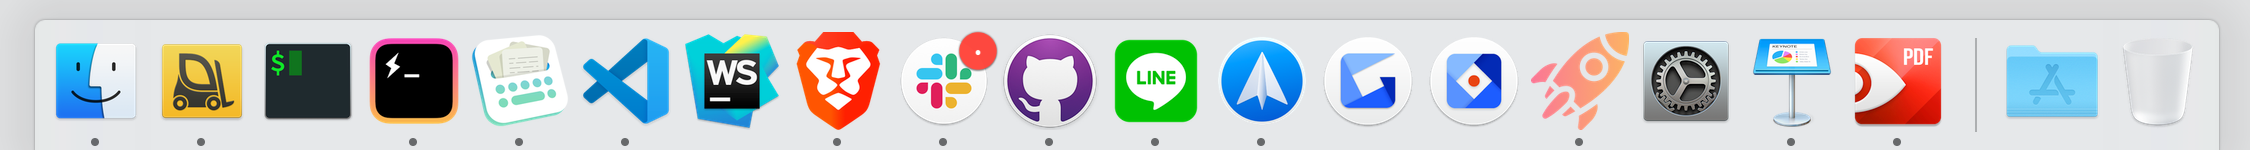
\includegraphics[width=100mm]{images/dock}}
    \end{center}
    \caption{Dock}
    \label{fig:dock}
\end{figure}

\subsubsection{メニュー型}

上述したDock等にメニューを設け、マウスを使用して登録したアプリケーションを起動できるようにする形式のランチャー。ホットキーと組み合わせて使用されるものもある。複数のアプリケーションを一つにまとめることで場所を節約できるだけでなく、階層化によって自分の使いやすいように整理することもできる。しかし、項目や階層が増えれば目的のアプリケーションに辿り着くまでの操作ステップは増えることになるため、稀に使用するアプリケーションを整理するために使うのが一般的である。

\newpage

\begin{figure}[h]
    \begin{center}
       \fbox{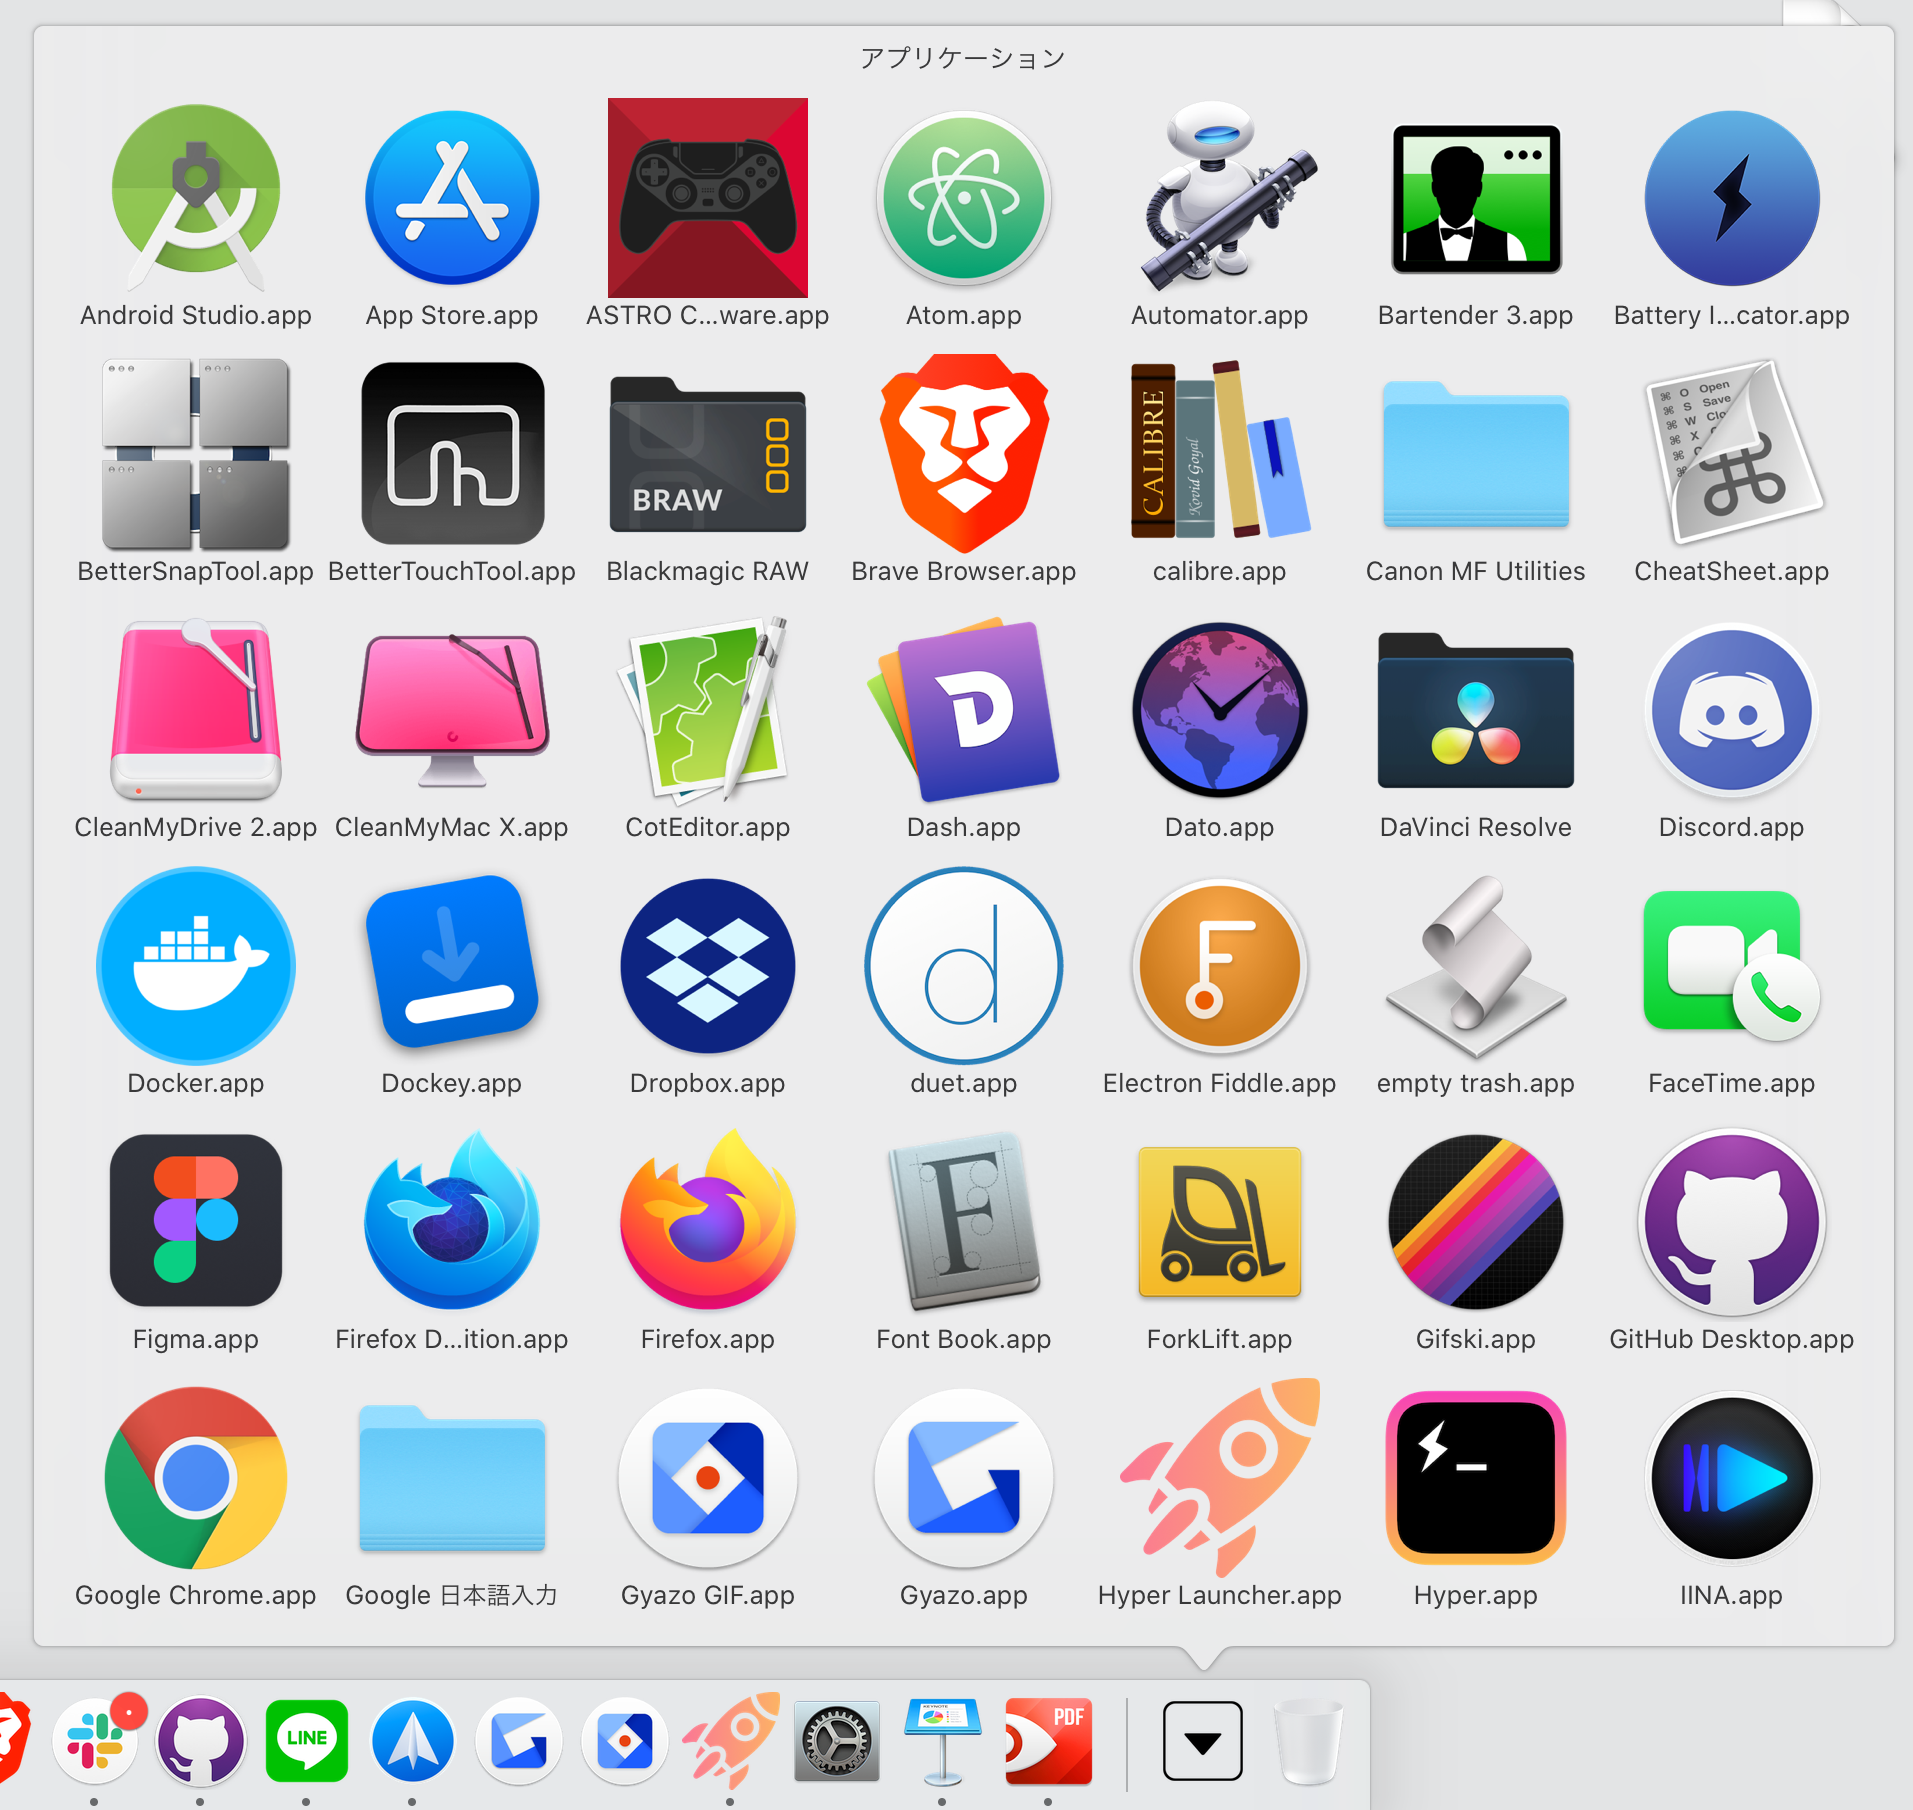
\includegraphics[width=100mm]{images/menu}}
    \end{center}
    \caption{Dock内のメニュー}
    \label{fig:menu}
\end{figure}

\subsubsection{検索型}

アプリケーションの名前を入力することで対象のアプリケーションを検索し起動する形式のランチャー。macOSにおけるSpotlightがこれにあたる。検索メニューは使用するときのみ表示されるため使用していない時は場所をとらないことに加え、キーボードのみで操作で完結するようになっている。もちろんマウスと組み合わせて使用することもできる。また大抵の場合インクリメンタルサーチが導入されているため、アプリケーションの名前を完全に覚えていなくても起動することができる。しかし、汎用性が高い反面、毎回一定のキーボード入力が必要となってしまうため、素早く複数のアプリケーションを切り替えるような操作には不向きである。

\begin{figure}[h]
    \begin{center}
       \fbox{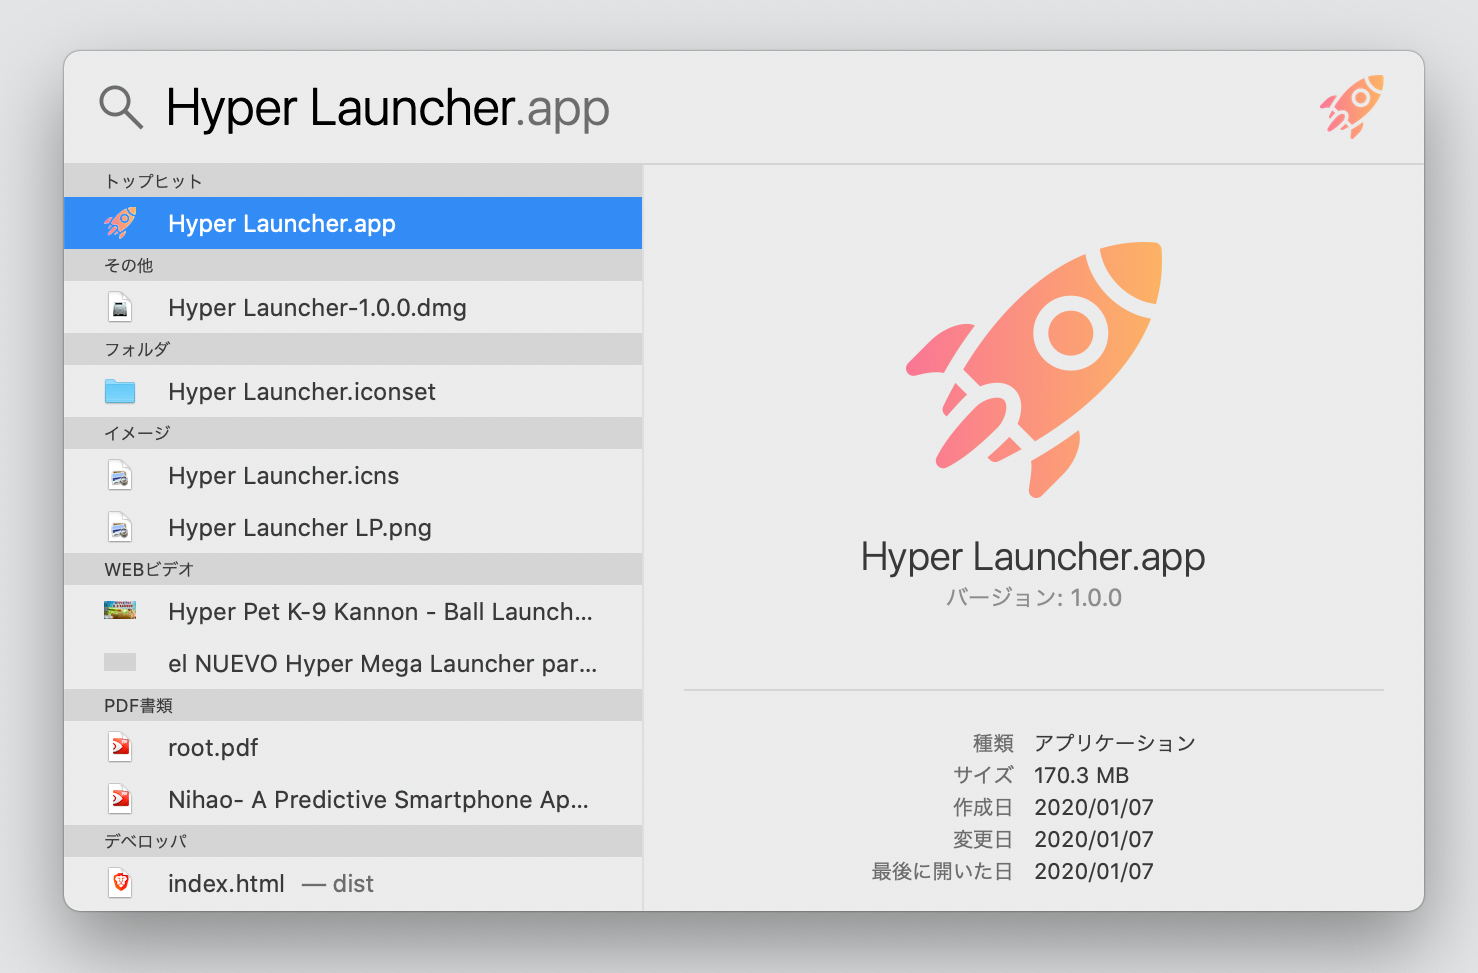
\includegraphics[width=100mm]{images/spotlight}}
    \end{center}
    \caption{Spotlight}
    \label{fig:spotlight}
\end{figure}

\subsubsection{ホットキー型}

単一のキーもしくは複数のキーの組み合わせを入力するだけで、登録したアプリケーションを起動できる形式のランチャー。他の形式のものとは違い、オペレーティングシステムに標準で搭載されていないことが多く、サードパーティ製ソフトウェアを自分で探す必要がある。普段は画面上に情報を表示する必要がないため場所をとらないが、その分どのホットキーにどのアプリケーションを登録したのか覚えておかなければならない。また、その設定画面のUIも使いやすいとは言えず、未習熟者には使いにくい形式だとされているのも事実である。
一発で特定のアプリケーションを起動できるというのはとても強力な機能ではあるが、あまり普及していないのはこれらの問題が原因だと考えられる。

\subsection{既存のアプリケーション}

先述した通り、ホットキーを利用したアプリケーションランチャーは標準で搭載されておらず、使用者自ら使いやすいものを探す必要がある。しかしその種類は豊富とは言えず、突出した特徴があるわけでもない。例として筆者が日常的に使用してきた2つのアプリケーションランチャーを示す。

\subsubsection{PMenu}

PMenu\footnote{https://danadesign.ltd/}(図\ref{fig:pmenu})はホットキーとメニューを利用したランチャーで、アプリケーションだけでなく様々なファイルをコマンドで操作することができる。使い勝手はいたって普通で可もなく不可もなくと言ったところである。自分の好きなホットキーを割り当てられるのは便利であるが、キーを登録するためのステップが多くとても煩雑で、こまめに切り替えるような使い方には向いていない。コンテキストメニューを利用することが主な方法とされているため、ホットキーに関しては最低限の機能が実装されているだけと言える。

\begin{figure}[h]
    \begin{center}
       \fbox{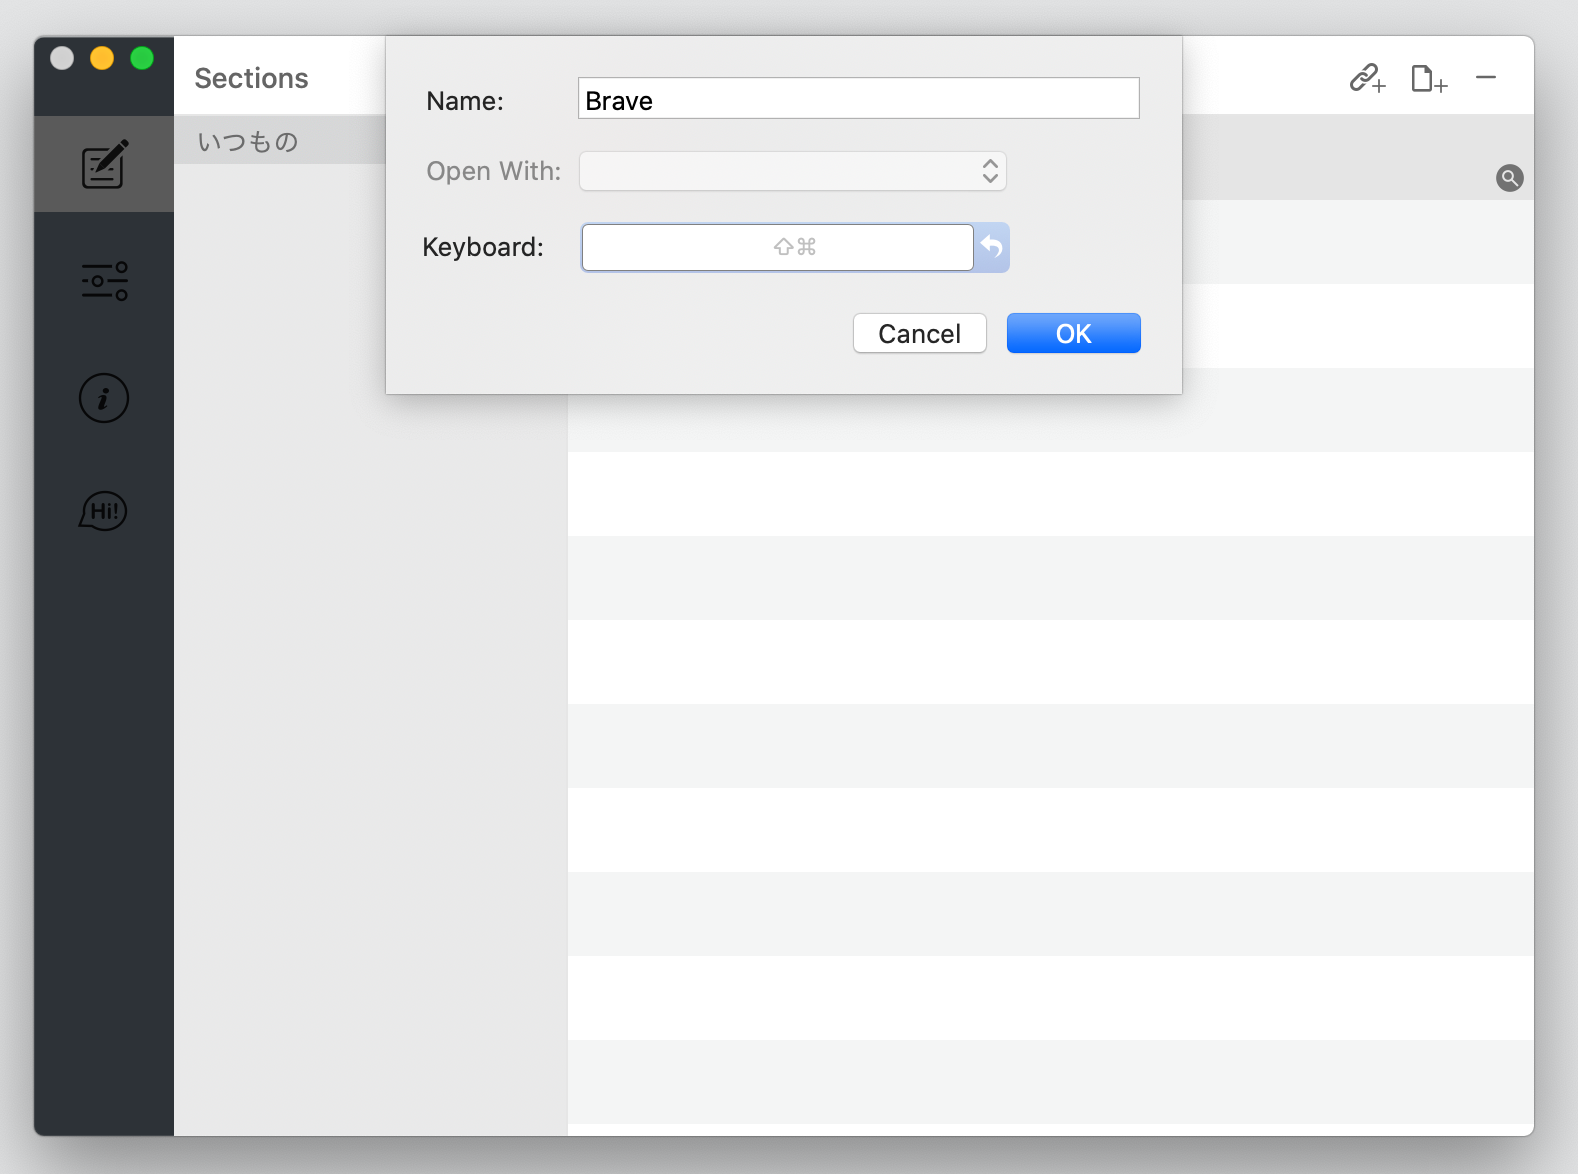
\includegraphics[width=100mm]{images/pmenu}}
    \end{center}
    \caption{PMenu}
    \label{fig:pmenu}
\end{figure}

\subsubsection{Snap}

Snap\footnote{https://apps.apple.com/jp/app/snap/id418073146}(図\ref{fig:snap})はホットキーを利用したランチャーで、macOSのDockを生かした機能が備わっている。SnapではDockに登録されたアプリケーションに左から順に数字を割り当てていき、その数字と設定したモディファイアキーとの組み合わせでアプリケーションを起動できるようになっている。これにより面倒な設定をすることなくホットキーの恩恵を授かることが可能となる。ただしDockのサイズは有限であり画面上に場所もとるため、多くのアプリケーションを登録するというのはあまり現実的ではない。ホットキーの設定も可能ではあるが、PMenuと同様操作ステップが多く使いやすいという印象は受けない。

\begin{figure}[h]
    \begin{center}
       \fbox{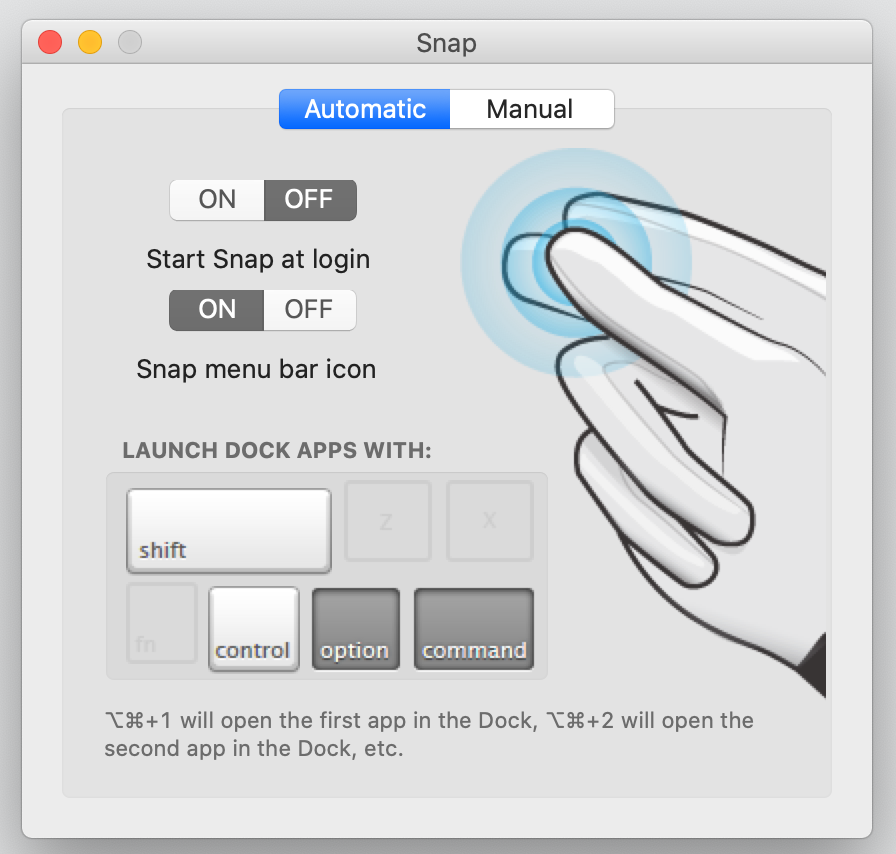
\includegraphics[width=100mm]{images/snap}}
    \end{center}
    \caption{Snap}
    \label{fig:snap}
\end{figure}

\subsection{ホットキー型の問題点}
このようにホットキー型のアプリケーションランチャーには設定の煩雑さや慣れるまでのハードルの高さなど、使いこなせるようになるまでに大きな障壁がある。また、その機能は強力であるものの、それ以上の特徴的な機能が搭載されることは少なく、改善の余地がたくさんあると考えられる。

\section{本研究の目的}
本研究の目的は、既存のホットキー型アプリケーションランチャーにおける不便を解消し、より強力でより多くの人に使いやすいシステムを開発することである。

\section{本論文の構成}

第1章では、本研究における背景と問題意識、目的について述べた。

第2章では、第1章で述べた問題意識を踏まえ、新しいホットキー型アプリケーションランチャーシステムを提案する。

第3章ではシステムの実装に関して述べ、第4章では関連研究について述べる。

第5章ではシステムの考察を行い、第6で本研究を総括する。  % 本文1
\chapter{システムの提案}
\label{chap:system}
本章では、アプリケーションランチャーについての背景を踏まえ、ホットキーを利用した新しいランチャーシステム「Hyper Launcher」を提案する。

\newpage

\section{設計}
既存のホットキー型アプリケーションランチャーに見られる不便を解消するため、

\begin{enumerate}
	\item アプリケーションの登録及びその変更が簡単にできる
	\item 設定が覚えやすい
	\item より強力に操作できる
\end{enumerate}

という3つの目標を実現するランチャーシステム「Hyper Launcher」を設計した。具体的には

\begin{enumerate}
	\item アプリケーションの登録や変更をドラッグアンドドロップによって簡単に行えるようにする
	\item 使用するホットキーの組み合わせを9つに制限し、そこに対してアプリケーションを登録することで、可能な限り認知不可を下げられるようにする
	\item 単一のホットキーの組み合わせに対して複数のアプリケーションを登録できるようにする
\end{enumerate}

というアプリケーションを実装した。

\section{基本操作}
自身の開発環境を考慮し、アプリケーションはmacOS上でデスクトップアプリとして利用できることとする。起動画面を図\ref{fig:hyper-launcher}に示す。
画面は9つのセクションに分けられており、予めそれぞれにホットキーが指定されている。

\begin{figure}[h]
    \begin{center}
       \fbox{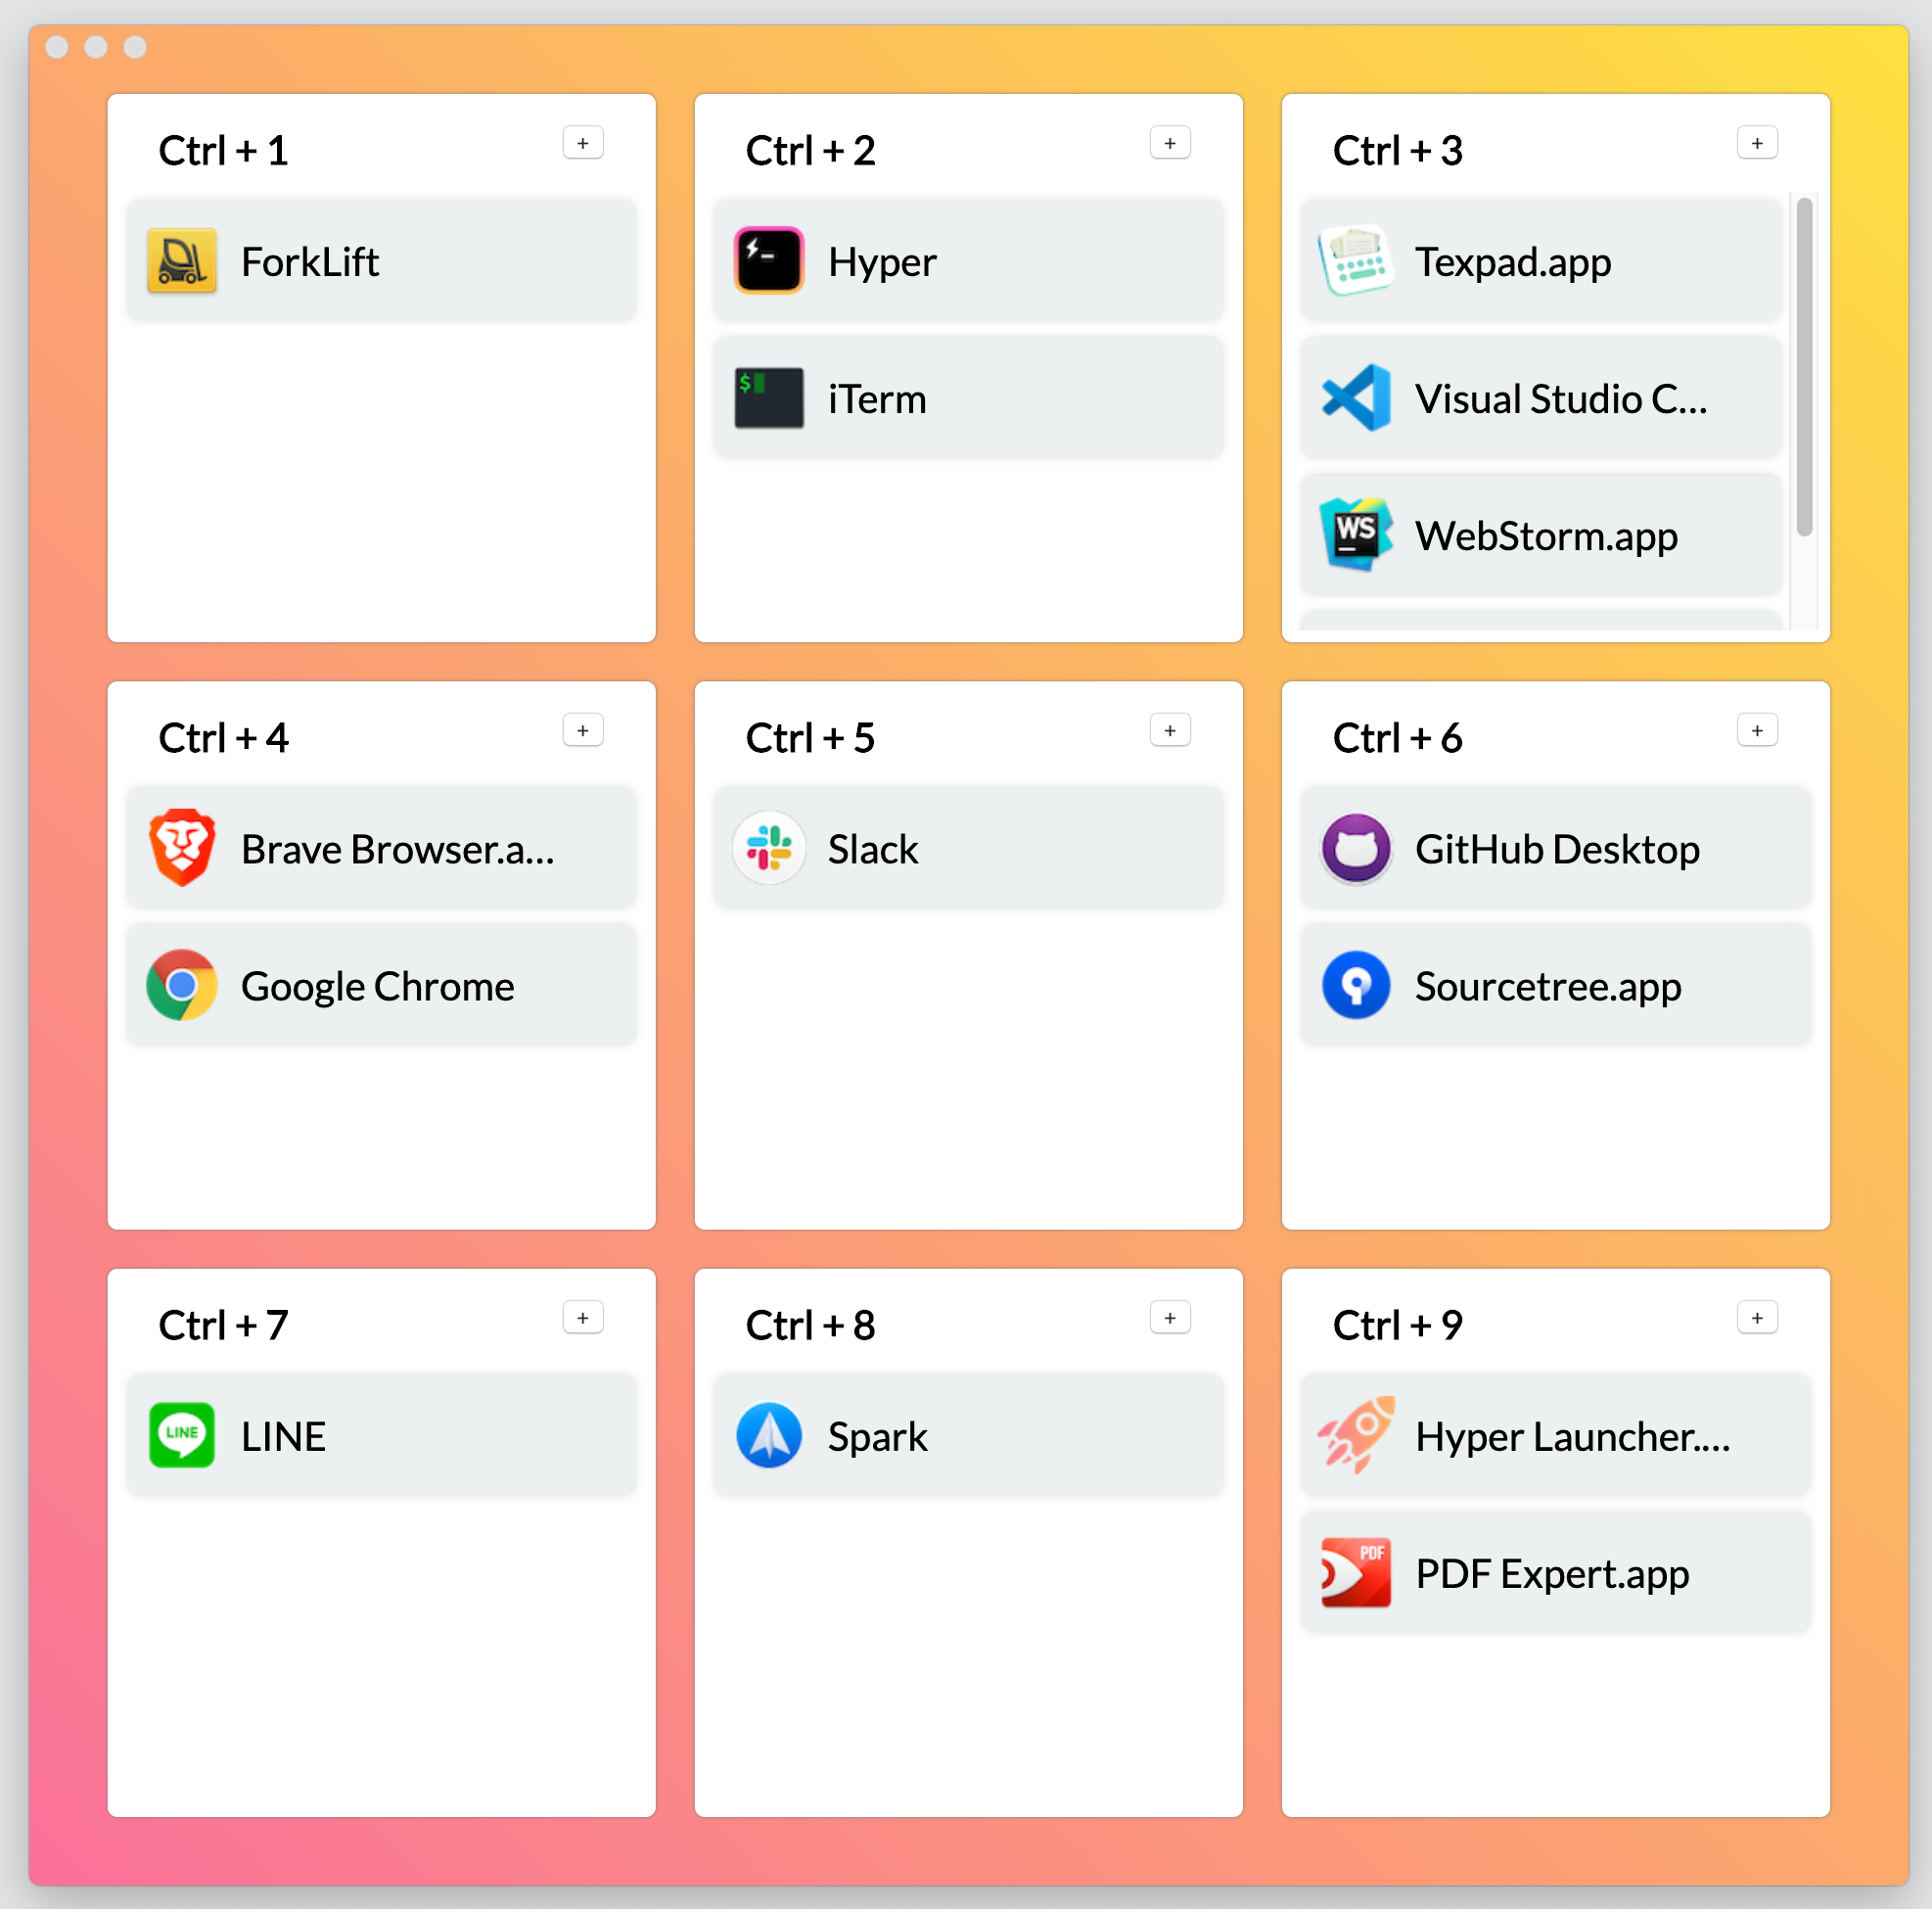
\includegraphics[width=100mm]{images/hyper-launcher}}
    \end{center}
    \caption{Hyper Launcherの起動画面}
    \label{fig:hyper-launcher}
\end{figure}

\subsection{アプリケーションの登録と起動}

任意のアプリケーションをそれぞれのセクションにドラッグアンドドロップすることで簡単に登録することができる。また、タイトル横のプラスボタンを押すことでアプリケーション選択画面が出現し、そこからも登録することができる。後は指定されたホットキーを入力するだけでアプリケーションを起動することができる。(図\ref{fig:add1}, \ref{fig:add2})

\begin{figure}[h]
    \begin{center}
       \fbox{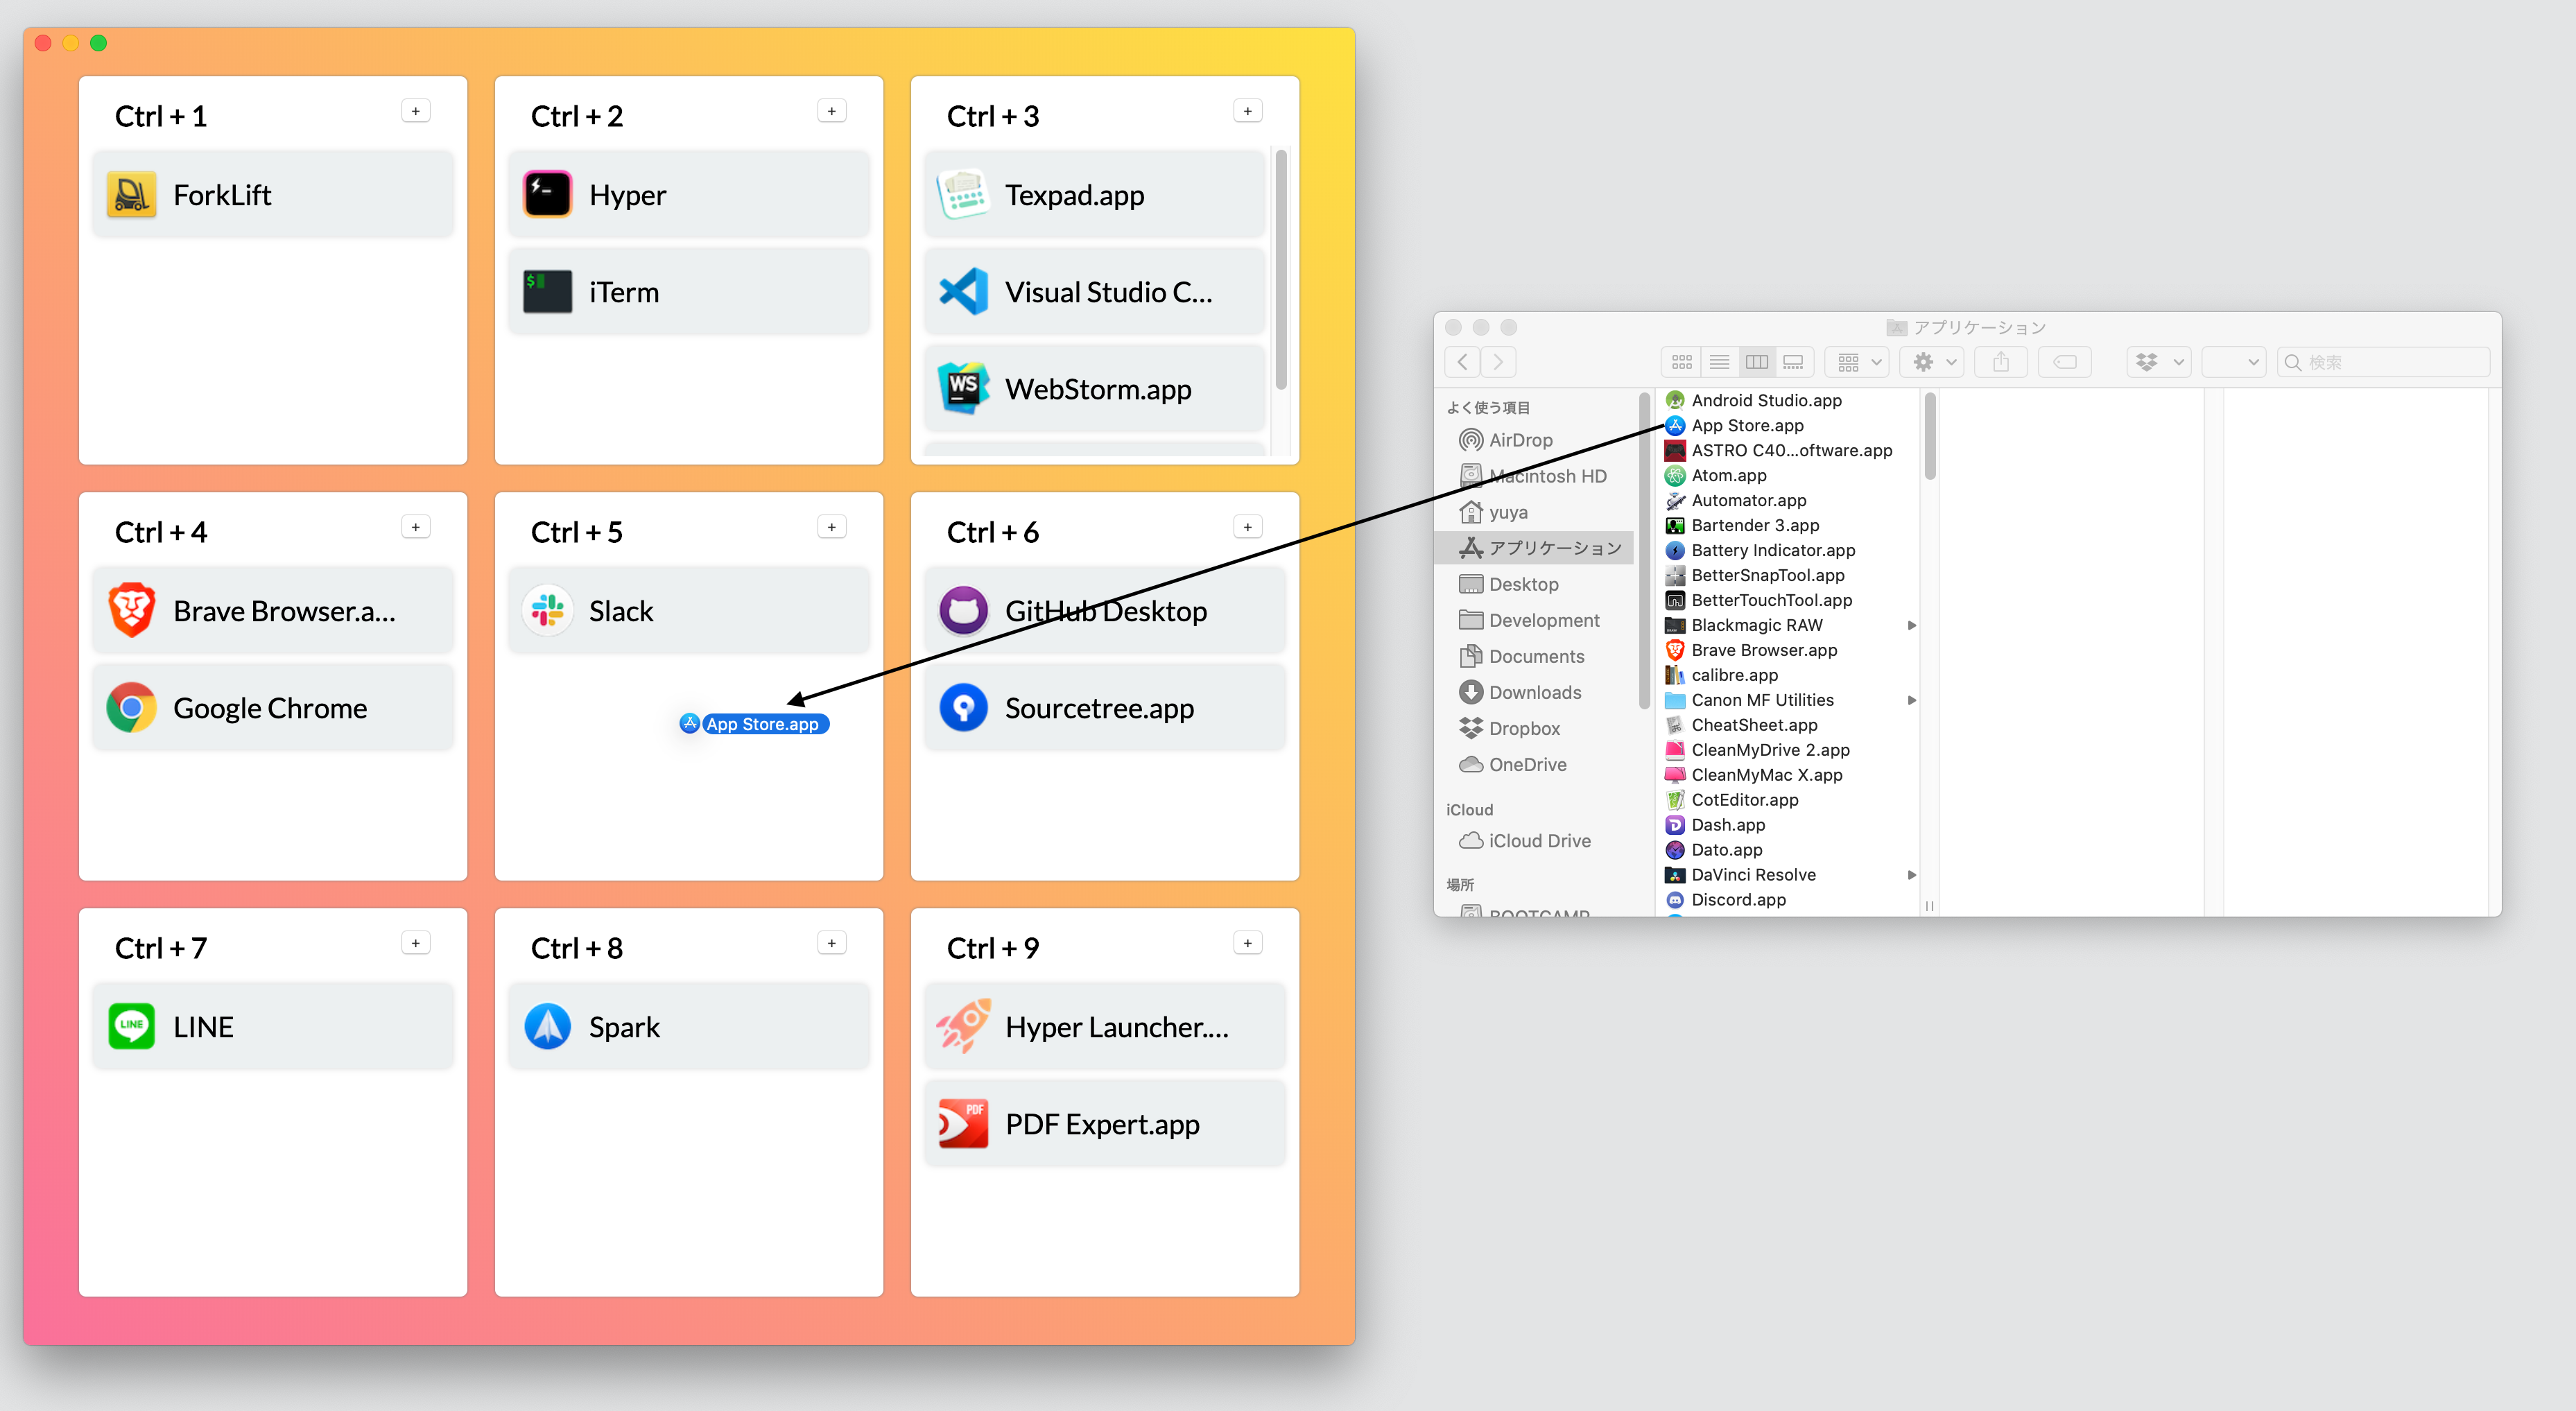
\includegraphics[width=100mm]{images/add1}}
    \end{center}
    \caption{ドラッグアンドドロップによる登録}
    \label{fig:add1}
\end{figure}

\begin{figure}[h]
    \begin{center}
       \fbox{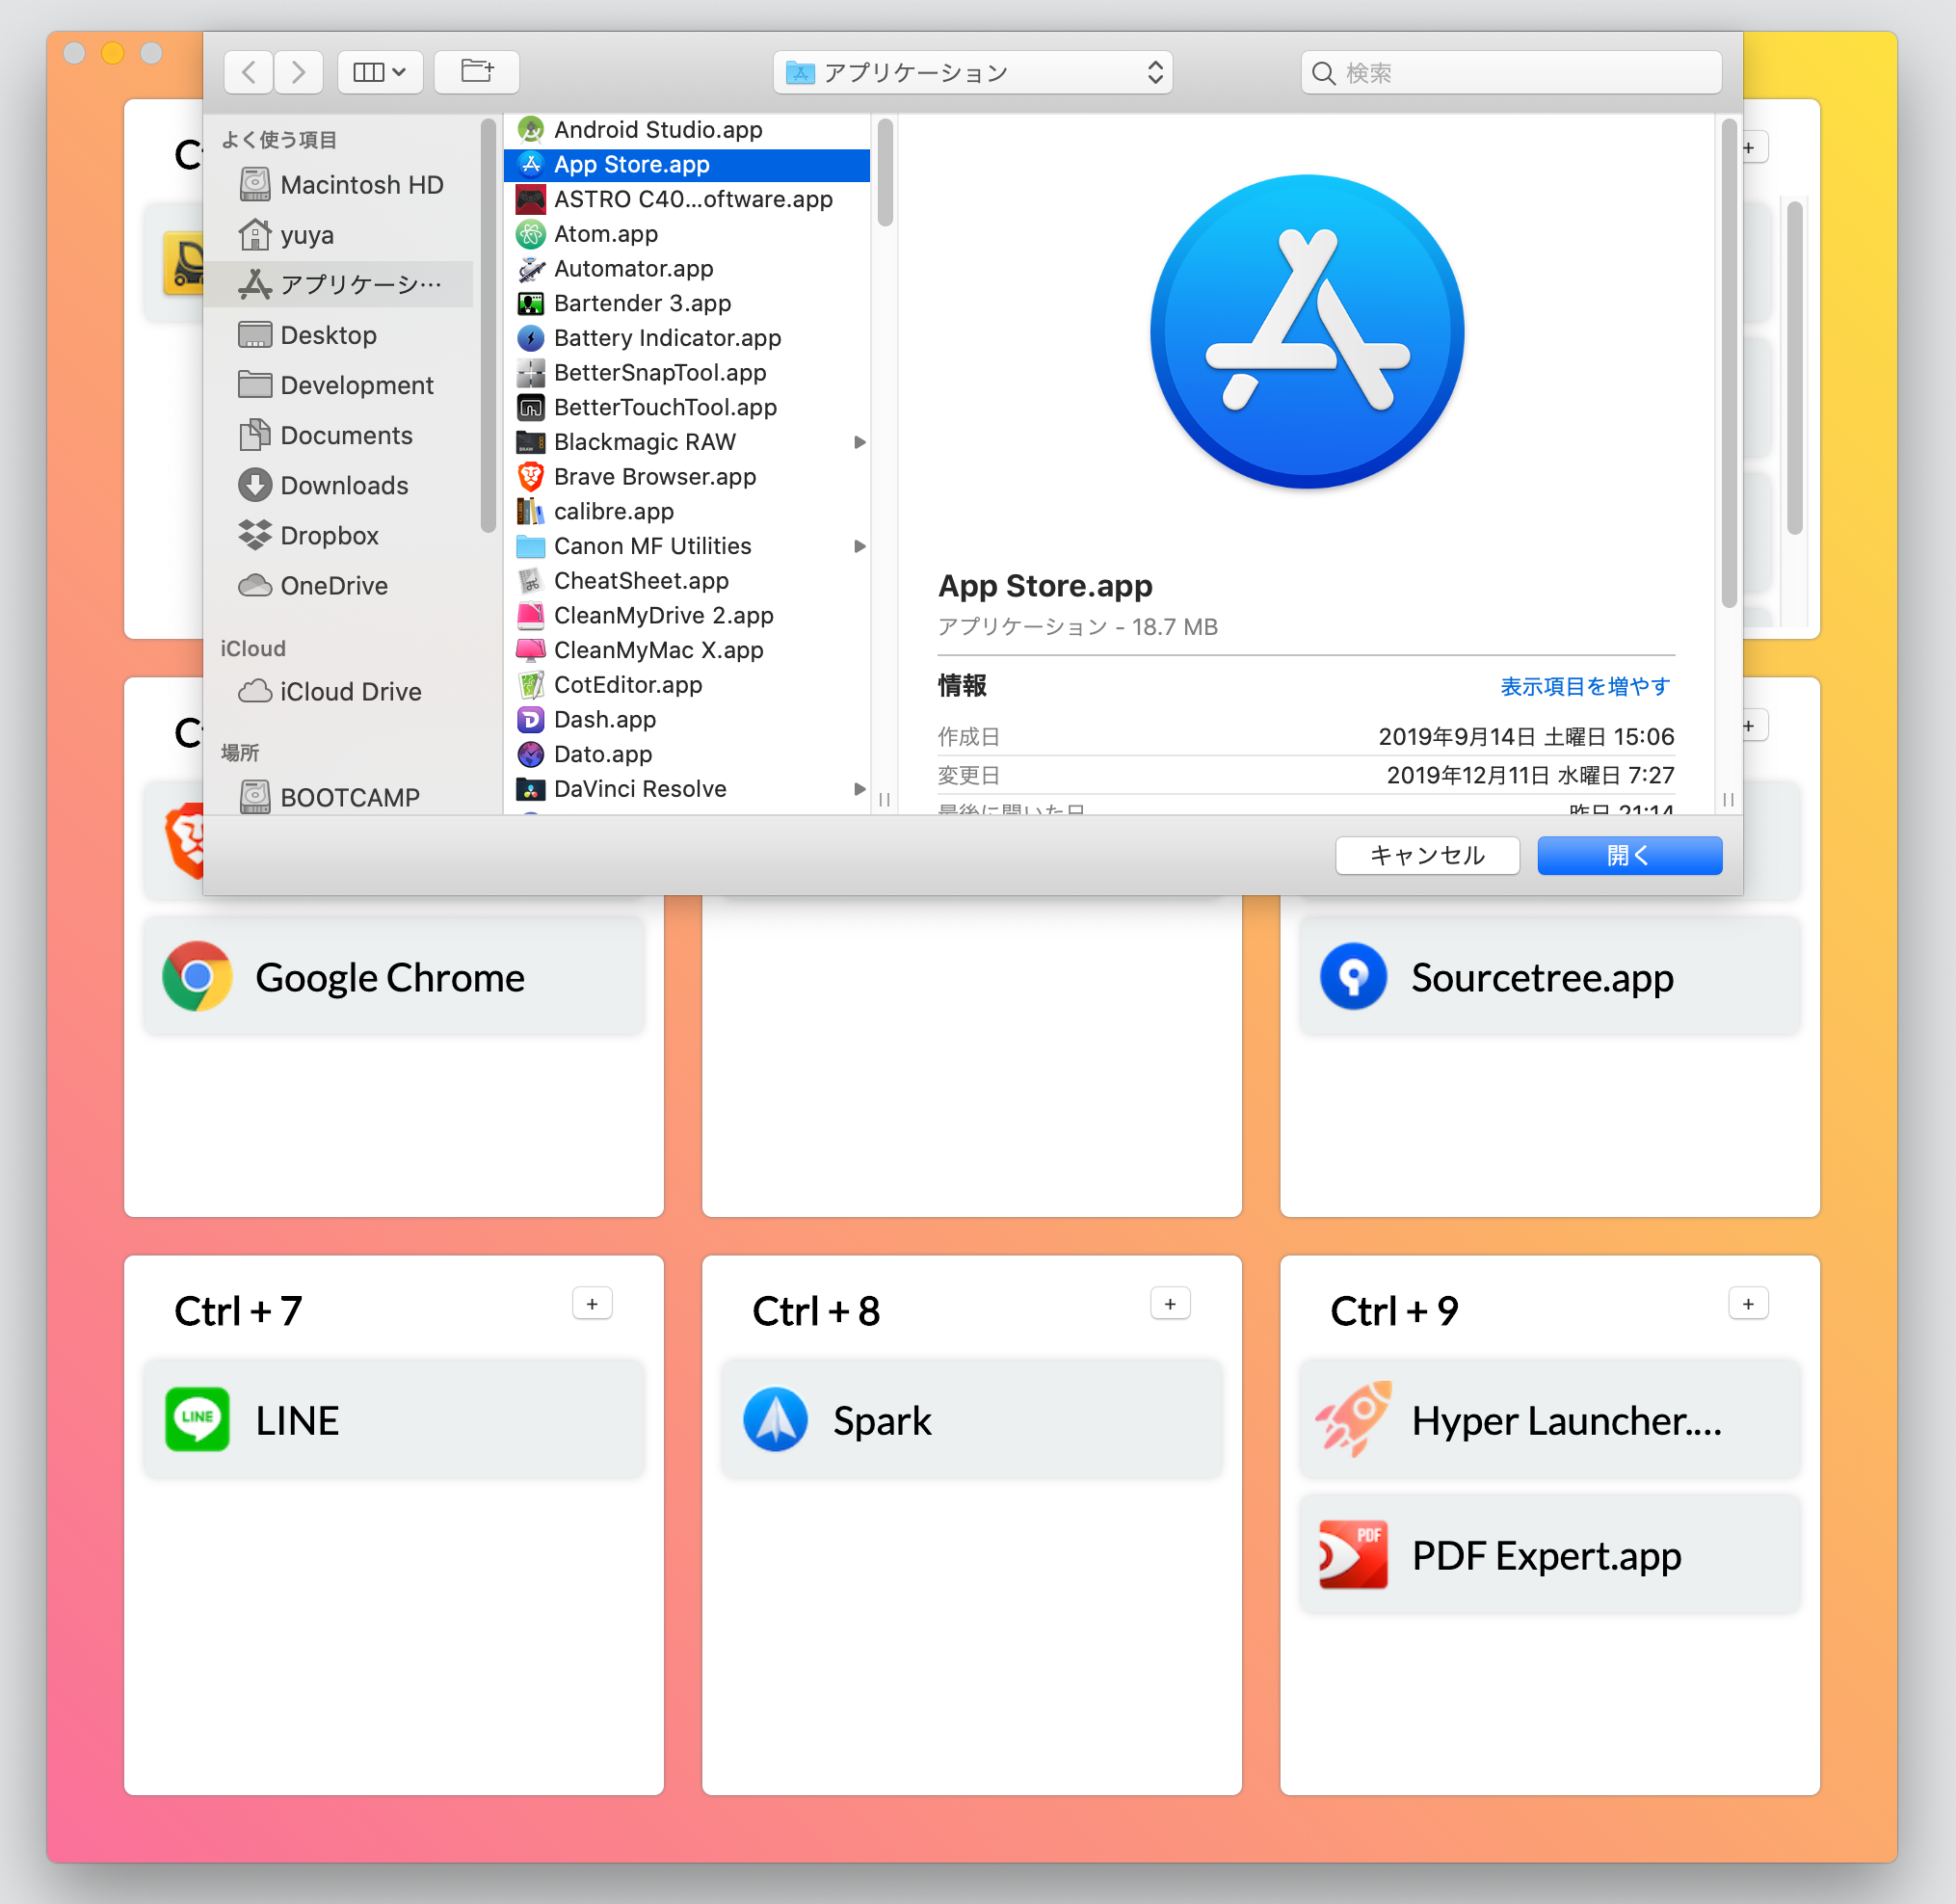
\includegraphics[width=100mm]{images/add2}}
    \end{center}
    \caption{追加ボタンから登録}
    \label{fig:add2}
\end{figure}

\subsection{アプリケーションの登録変更と解除}
アプリケーションに紐付けるホットキーを変更したい時は、対象のアプリケーションを目的のセクションへドラッグアンドドロップするだけで操作が完了する。またアプリケーションにマウスカーソルを乗せた際に右側に表れる削除ボタンを押すことで、登録を解除することができる。(図\ref{fig:change}, \ref{fig:delete})

\begin{figure}[h]
    \begin{center}
       \fbox{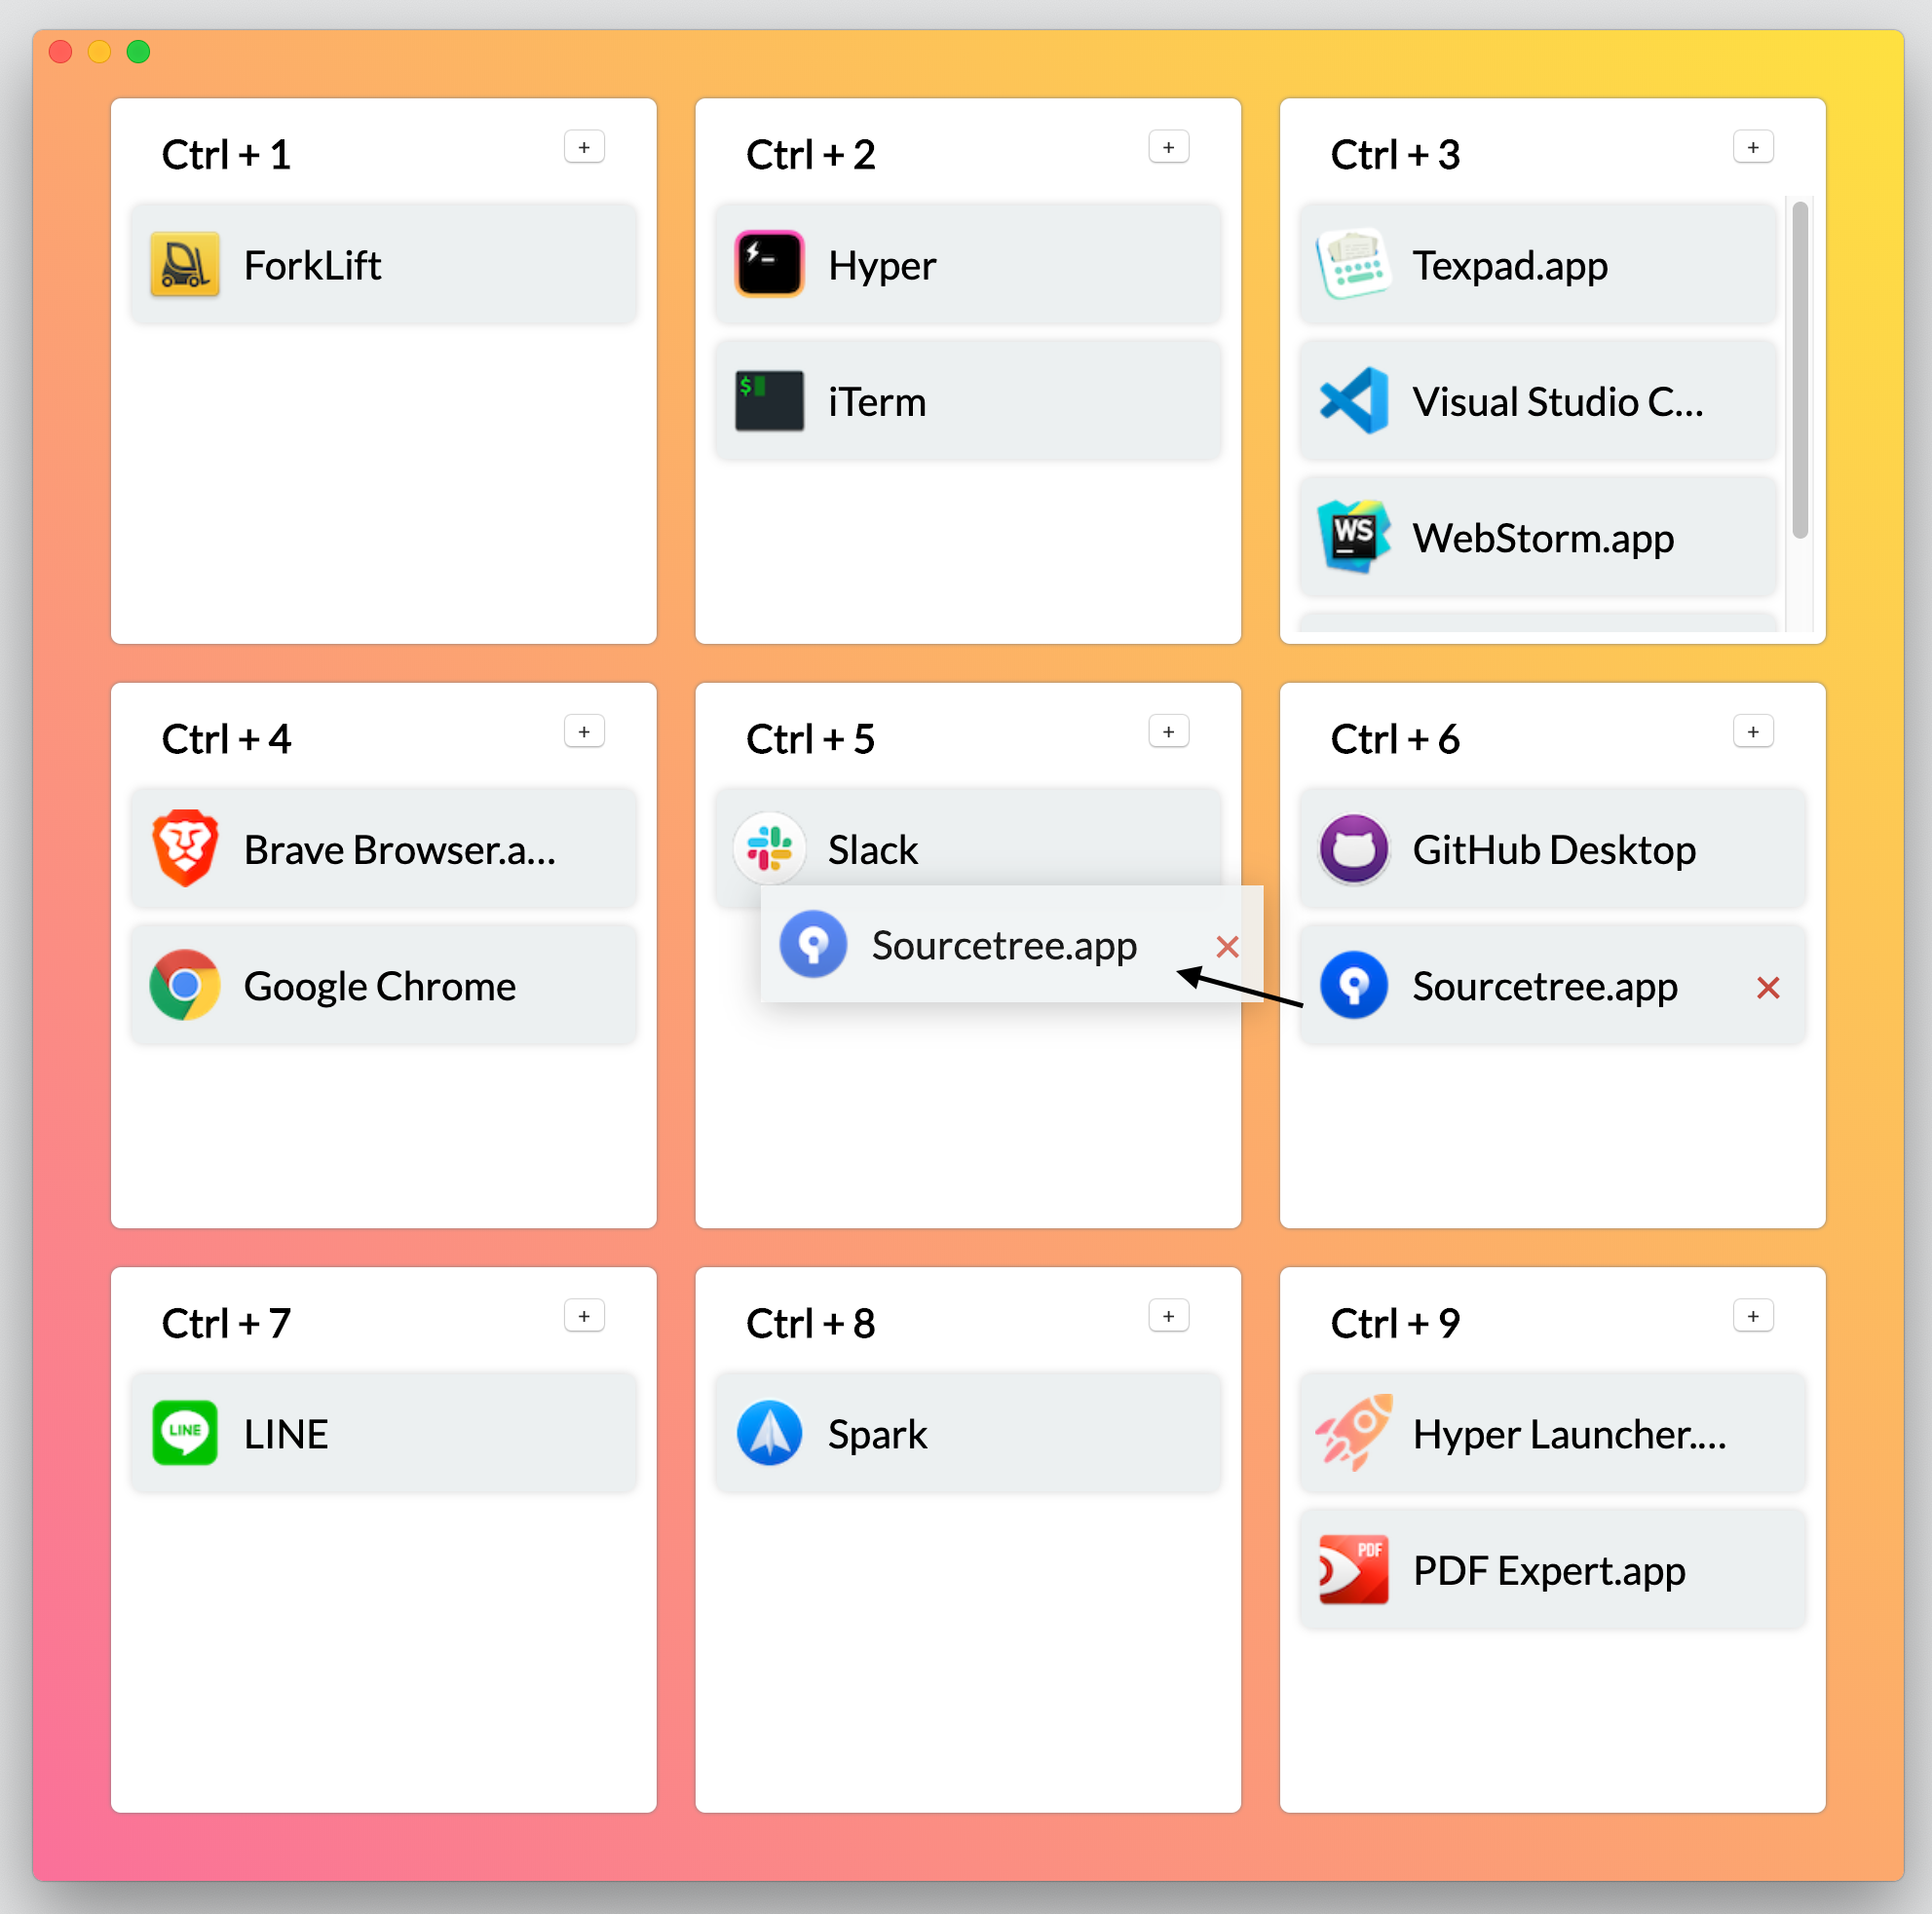
\includegraphics[width=100mm]{images/change}}
    \end{center}
    \caption{登録の変更}
    \label{fig:change}
\end{figure}

\begin{figure}[h]
    \begin{center}
       \fbox{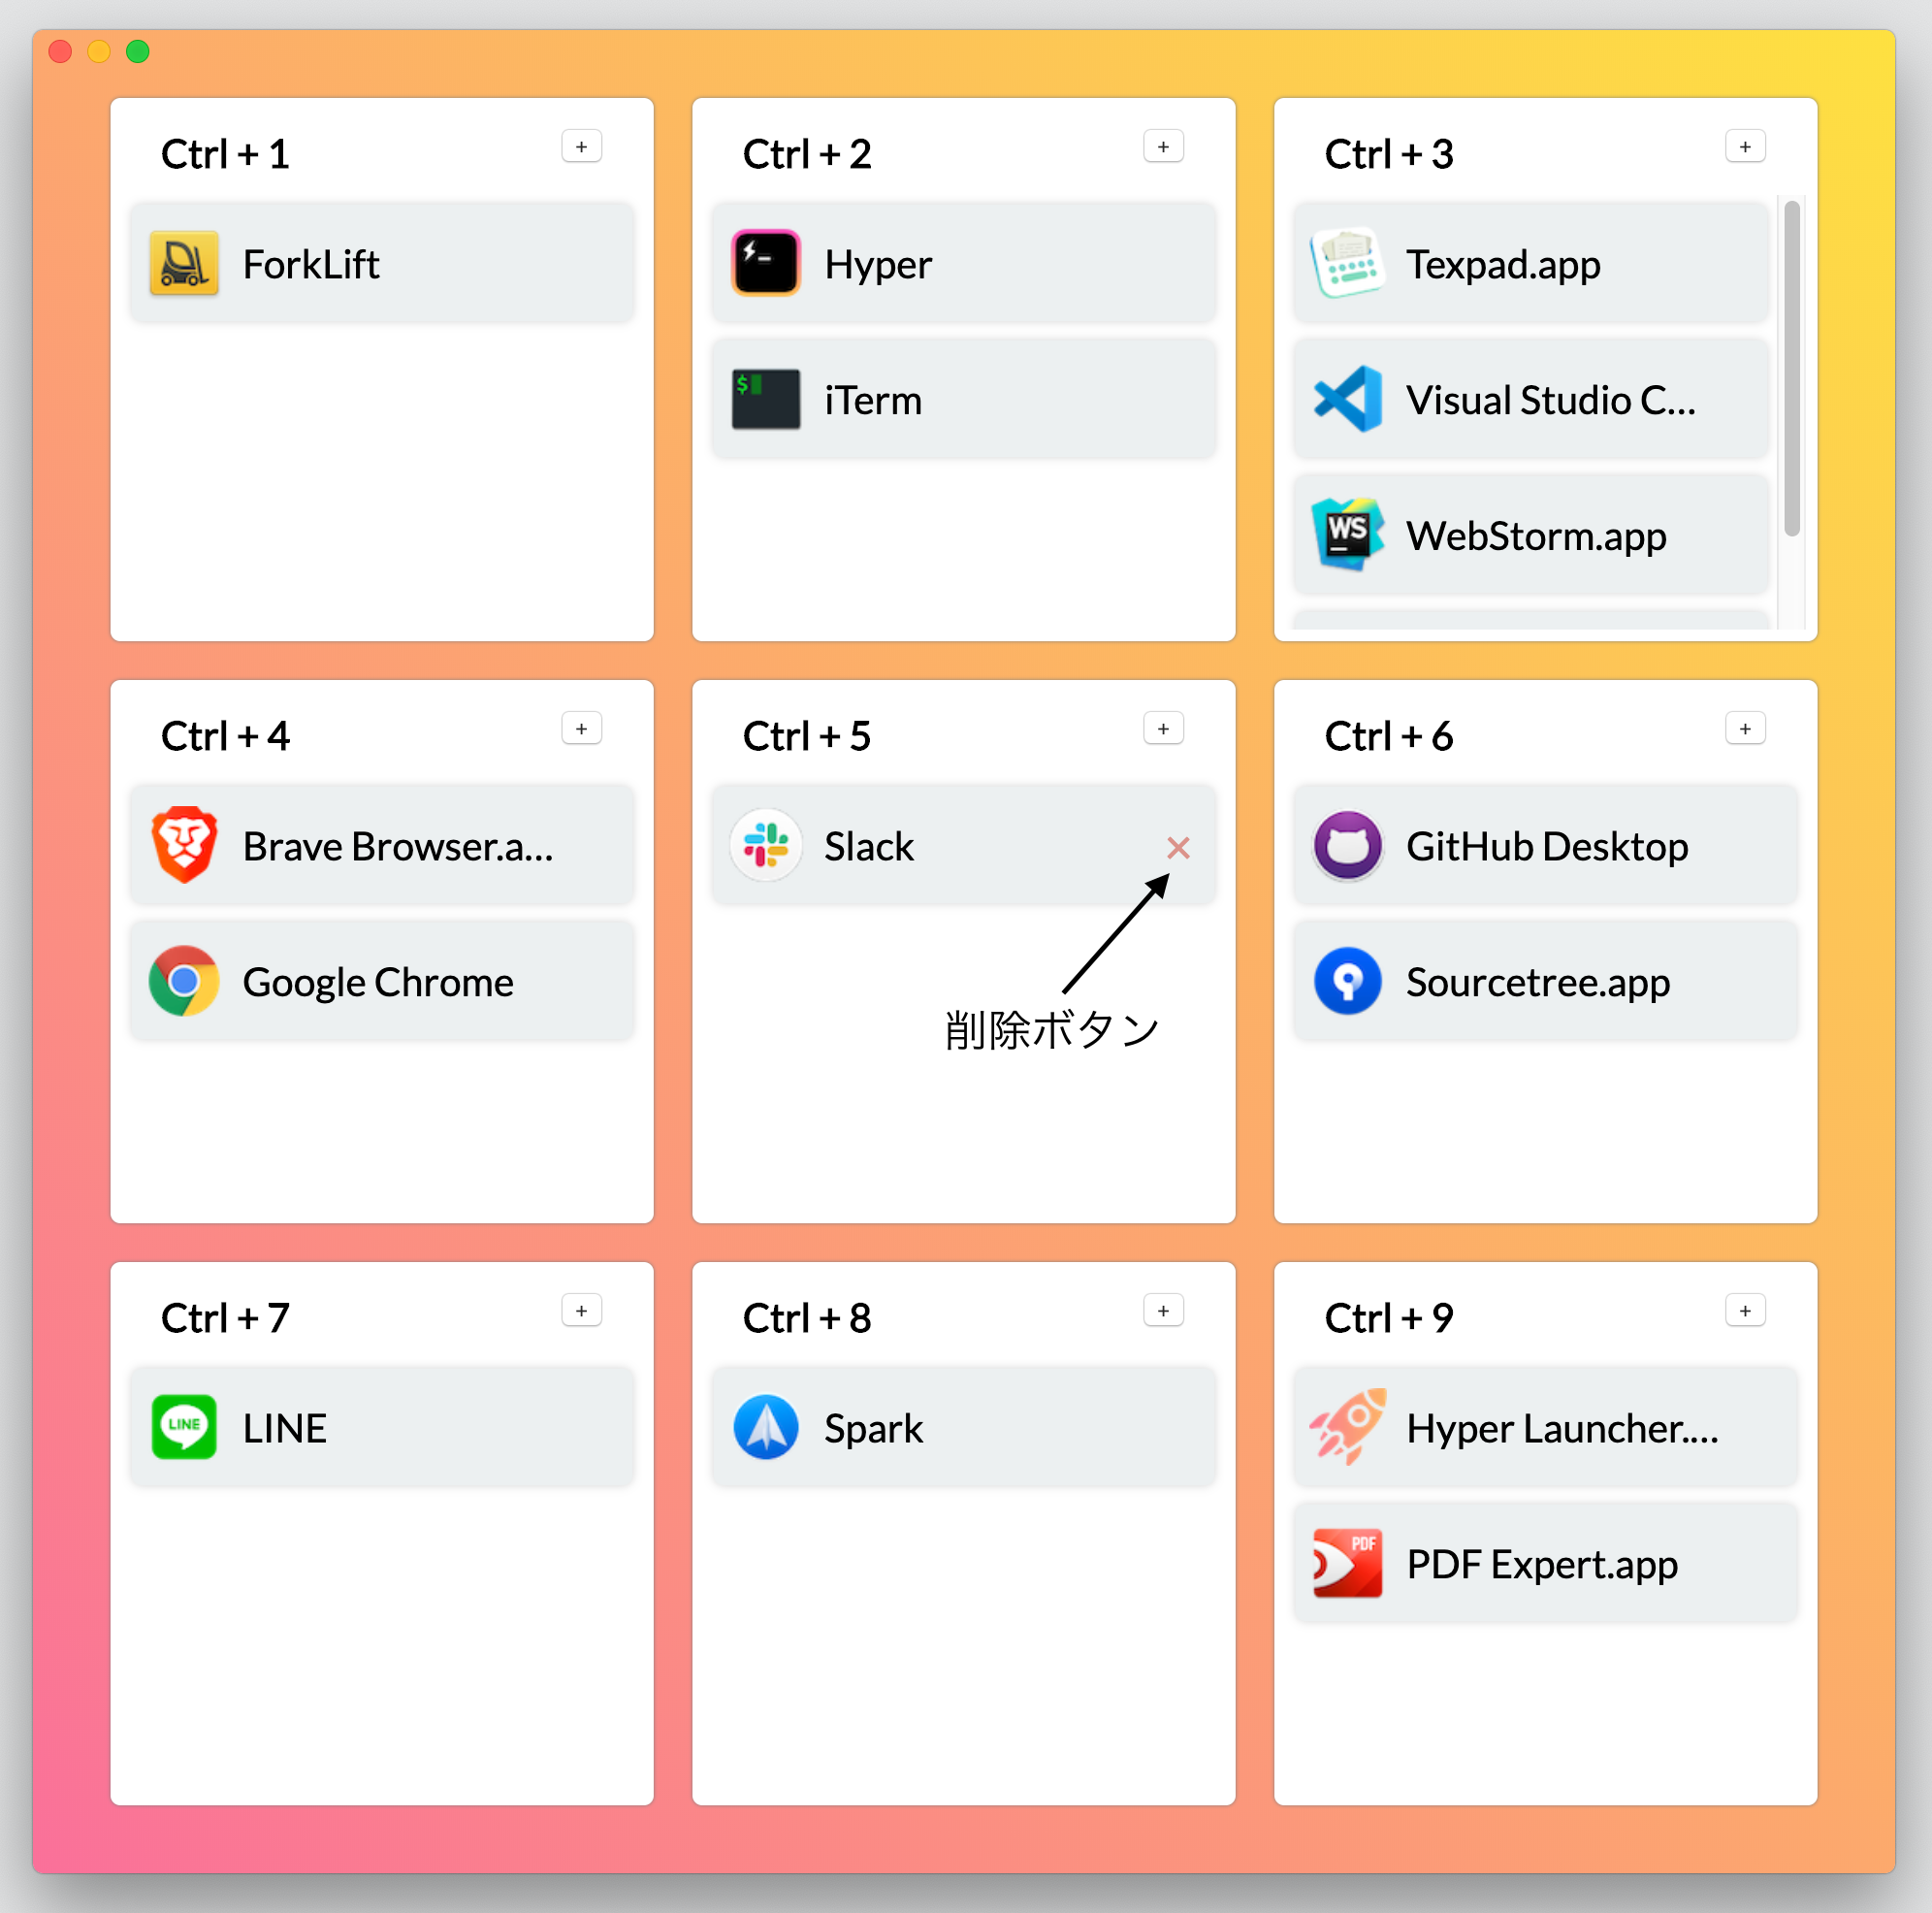
\includegraphics[width=100mm]{images/delete}}
    \end{center}
    \caption{登録の解除}
    \label{fig:delete}
\end{figure}

\subsection{複数アプリケーションの登録と操作}
既にアプリケーションが登録されているセクションに、同じように新しいアプリケーションを追加するだけで複数のアプリケーションを登録することができる。アプリケーションは表示されている順番によって優先順位が定められており、キーを入力する度にその優先順位に基づき順番に起動するようになっている。その優先順についてもドラッグアンドドロップするだけで変更することができる。  % 本文2
\chapter{実装}
本章では、第2章で述べたシステムの設計を受け、Hyper Launcherの実装について述べる。

\newpage

\section{システム構成}
Hyper Launcherはユーザーがアプリケーションを登録するためのクライアントと、登録したデータを保存しておくためのデータストアから構成される。構成図を図\ref{fig:system}に示す。

\begin{figure}[h]
    \begin{center}
       \fbox{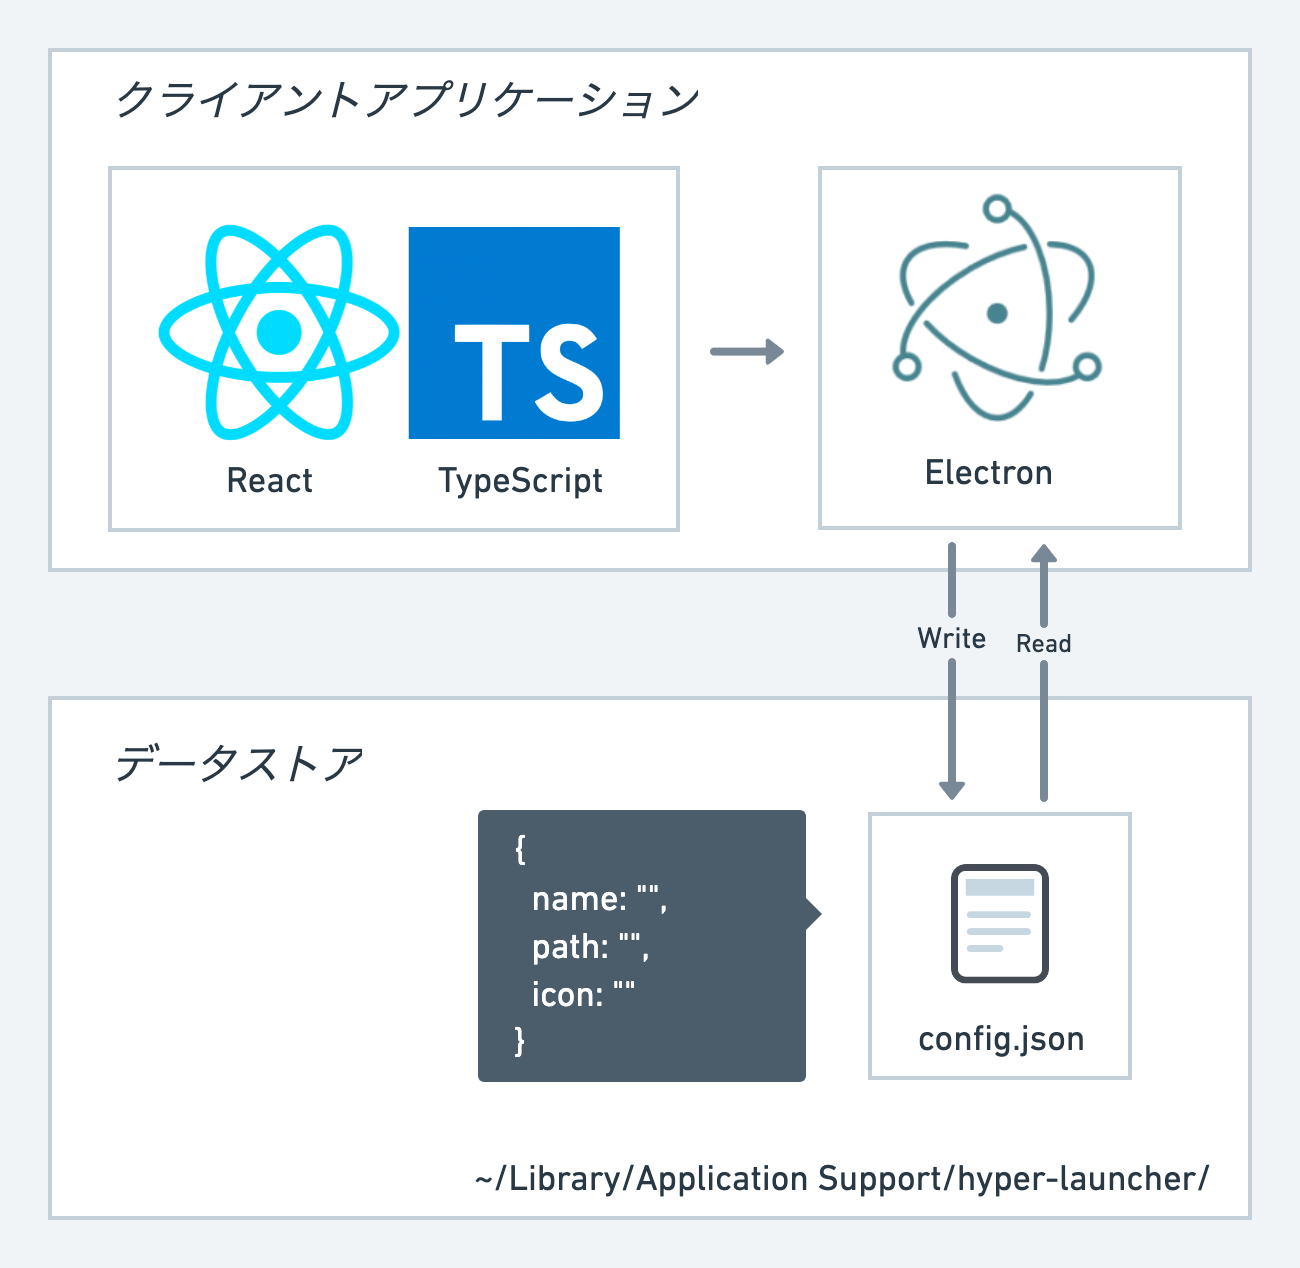
\includegraphics[width=100mm]{images/system}}
    \end{center}
    \caption{システムの構成}
    \label{fig:system}
\end{figure}

\section{クライアント}
クライアントはElectron\footnote{https://electronjs.org}やTypeScript\footnote{https://www.typescriptlang.org/}、React\footnote{https://reactjs.org}といったWeb技術によって実装されており、macOSのデスクトップアプリケーションとして動作する。

\subsubsection{Electron}
ElectronはHTML、JavaScript、CSSを用いてクロスプラットフォームなデスクトプアプリケーションを作成することができるソフトウェアフレームワークである。Electron自体はChromiumとNode.jsを使用しておりWeb技術のみで開発が完結するのが利点である。Hyper LauncherではElectronのglobalShortcutというAPIを利用し、Hyper Launcherが非アクティブ状態でもホットキーの入力を取得できるようになっている。アプリケーションの起動やアクティブ化なども標準の機能だけで実装できるため、ランチャーに適したフレームワークと言える。

\subsubsection{AppleScript}
Web技術のみでは実装が難しい部分についてはAppleScriptを使用した。masOSにはosascriptと呼ばれるシェルスクリプトが存在し、これを利用することでNode.js\footnote{https://nodejs.org}からAppleScriptを実行することができる。AppleScriptによって、起動中のアプリケーションや特定のアプリケーションがアクティブかどうかといった情報を取得することができ、これによってデスクトップアプリケーションとして十分な機能を実装することが可能となった。ただし実行する毎にプロセスを立ち上げるため、無闇に使用してしまうとラグが発生してしまう。また、AppleScriptはmacOSのみで使えるものであるため、Electronの利点であるクロスプラットフォーム対応はできなくなってしまった。

\section{データストア}
ユーザーが登録した情報は、Electronが定義するユーザーデータ領域(~/Library/Application Support/hyper-launcher/)にJSONファイルとして保存されている。データのやり取りが全てローカルで完結するため、オフラインでも使用できようになっている。データはホットキーの数字をキーにしアプリケーション情報の配列を値として持ったオブジェクトになっており、アプリケーション情報にはアプリケーションの名前、パス、そしてbase64エンコードされたアイコンの3つが含まれている。これにより単一のキーに対して複数のアプリケーションを登録することが可能となっている。以下にその例を示す。ただしiconのbase64文字列と中間部分は長くなるため省略した。

\begin{lstlisting}[caption=config.json]
{
  "shortcut": {
    "1": [
      {
        "name": "ForkLift",
        "path": "/Applications/ForkLift.app",
        "icon": "***************************"
      }
    ],
    "2": [
      {
        "name": "Hyper",
        "path": "/Applications/Hyper.app",
        "icon": "***************************"
      }
    ],
    
    ・・・
    
    "9": [
      {
        "name": "Hyper Launcher",
        "path": "/Applications/Hyper Launcher.app",
        "icon": "***************************"
      }
    ],
  }
}
\end{lstlisting}  % 本文3
\chapter{実運用及び評価}
本章では、Hyper Launcherを実際に運用した結果および評価について述べる。

\newpage

\section{筆者の運用}
筆者は本システムを開発段階を含め半年以上利用した。日常的にホットキー型のランチャーを使用しているため覚えやすについての評価は出来ないが、その他については大きな利点を実感することができた。特に登録の作業は格段に便利になった。今まではアプリケーションを選択した後に割り当てるキーを選択する必要があったが、そのフローが一つにまとめられたことにより、余計なことを考える必要がなくなった。また一つのホットキーに対して複数のアプリケーションを登録できるため、これまで以上に柔軟な操作が可能となった。1~9に対してカテゴリーごとに分けてアプリケーションを管理し状況に応じてそれらを使い分けたり、よく使うアプリケーションの組み合わせを一つのホットキーにまとめたりと活用の幅が広がった。ただし、複数登録の操作についてはまだまだ改善の余地があると考えられる。

\section{第三者の意見}
研究室のメンバーのうち、ホットキー型のランチャーをあまり使ったことのない2名に実際に利用してもらった。

\subsection{アプリケーションの登録について}
アプリケーションの登録にドラッグアンドドロップを採用した点については好意的な意見が得られた。普通は面倒な作業でもHyper Launcherでは楽しく設定できるようになっていると評価できる。また事前にホットキーがしていされているということも、設定の敷居を下げている要因の一つになっている。ランチャーに限らずホットキーを登録するインターフェースは煩雑なものが多いため、これは大きなアドバンテージだと考えられる。

\subsection{ホットキーの覚えやすさについて}
設定自体は簡単になっていたが、覚えやすさという点ではまだまだ難しいという意見が得られた。事前にホットキーが固定されてはいるものの、そのホットキーとアプリケーションの対応を覚えなければならないことには変わらず、ホットキーの使用に慣れていない人にとっては依然として敷居が高いということがわかった。

\subsection{ホットキー自体の有用性について}
今回はホットキー型のランチャーをあまり使ったことのない人に試してもらうことができたが、しばらく使っていく中でその便利さを実感してもらうことができた。特にホットキーの入力一発で素早く起動できるという点は好評だった。しかし今後も使用を続けるかとなるとまだ障壁があり、初心者でも段階的に使いやすくなっていくような仕組みが必要なのではないかと感じた。

\subsection{問題点}
その他、細かい問題点についても意見が得られた。以下にそれを示す。
\begin{itemize}
  \item 複数登録している場合の操作がわかりづらい。直感的でない。
  \item 削除時の確認はいらない。不可逆の変化ではないので簡単に消せたほうが良い。
  \item ドラッグアンドドロップの移動にバグがある。
  \item MacBookの場合小指で入力する必要があるため、Controlキーの入力が難しい。
\end{itemize}
これ以外にも痒い所に手が届かないという指摘はいくつかあり、そういった部分については個別にカスタマイズできるような仕組みが必要であると感じた。  % 本文4
\chapter{議論}
本章では、Hyper Launcherについての議論を行う。

\newpage

\section{関連研究}
Hyper Launcherを設定するにあたり、参考になった文献について述べる。

\subsubsection{macOSでディスプレイ1枚で作業する技術}
これは筆者が感銘を受けた記事\cite{onedisplay}の一つで、ホットキー型ランチャーの習得を始めるようになったきっかけでもある。記事中ではノートパソコンの小さい画面で如何に複数のアプリケーションを切り替えて操作していくかということが詳細に述べられており、そのキーの設定や思想はHyper Launcherを設計する上で大きく影響を受けた。特に、画面を10個に分割するという考えた方は、ホットキーを予め9つに制限するという方法に繋がり、とても参考になった。

\subsubsection{FALCON}
FALCON\cite{falcon}はスマートフォン向けのアプリケーションランチャーで、ユーザーが次に使用する確率の高いアプリケーションを、ユーザーのいる場所や普段の傾向といったコンテキストから予測し推薦してくれるというシステムである。予測をしてアプリケーションを並び替えて推薦するという手法は、スマートフォンのようにアプリケーションが格子状に並んでいる場合には効果的であるといえる。ホットキーと組み合わせると、一つのキーのみで複数のアプリケーションが操作できるようなインターフェースができるかもしれないと考えられる。しかし、完璧な予測モデルを作成するのは困難であり、今回は一つのキーに複数のアプリケーションを登録できるようにすることで、その機能に近づけられるよう工夫した。

\subsubsection{HotStrokes}
HotStrokes\cite{hotstrokes}はホットキーの有用性を認めつつより習得しやすく且つGUIメニューよりも効果的な手法として、トラックパッドを利用したジェスチャによるコマンド入力を提案している。確かに視覚的に記憶しやすいジェスチャをコマンドに対応させるという試みは興味深いが、トラックパッドが使える環境は限られており、ホットキーに比べ汎用性に劣ると考えられる。インターフェースの大きな変革がない限り、ホットキーの習得をサポートするような手法を取り入れるほうが効果的だと考える。

\subsubsection{IconHK}
IconHK\cite{iconhk}はツールバー上のボタンアイコンにホットキーに関する情報を埋め込むことで、ユーザーの覚えやすさを補助しようというシステムである。ホットキー型のアプリケーションランチャーの場合、画面に表示するものは基本的に何もないため、直接的に取り入れることはできなかったが、これを機にユーザーに寄り添うための機能が必要だと考え始めた。IconHKはその使いやすさとアプリケーションとしての見た目を損なわずに済むという利点を兼ね備えており、これはデスクトップ上に情報を埋め込むなどの方法で応用できるかもしれない。

\subsubsection{ExposeHK}
ExposeHK\cite{exposehk}はホットキーの使用を助けるシステムで、モディファイアキーを長押しすることで対象アプリケーションに割り当てられているホットキーをツールバー上にプレビューできるというものだ。これにより非習熟者であっても段階的にホットキーを覚えていくことが可能となる。このようなプレビュー機能については実際に使ってもらった中でも欲しいという意見があった。Electronでは長押しの実装ができず断念したが、この機能の重要性は高いと言える。プレビューの表示方法についても様々なバリエーションが考えられ、全てを羅列するだけでなく隣接するホットキーの情報を表示するなどHyper Launcherに最適な方法を模索したい。

\subsubsection{FingerArc, FingerChord}
FingerArc及びFingerChord\cite{fingerarcandfinderchord}はホットキーの習熟をサポートするシステムである。カメラを利用して指の位置やその動きを認識し、関連するホットキーを表示してくれるようになっている。これにより非習熟者でも視覚的なガイダンスを通じてマッピングを学習できるようになっている。このような習熟をサポートするシステムは数多く提案されているが、カメラやセンサを使った比較的大掛かりな手法はあまり受け入れられないのではないかと考える。まずはホットキーの便利さを実感してもらえるよう導入の敷居を下げ、そこから使いこなしていけるようにサポートするようなシステムが必要である。


\section{展望}

\subsubsection{ネイティブアプリケーション}
今回は筆者のスキルの都合上Electronを使用した開発になったが、やはりネイティブアプリケーションと比べると実装に限界を感じる部分があった。今後様々なインターフェースを試していくためには、Swift等を利用したより高度が開発が求められる。

\subsubsection{習熟のサポート}
実際に使用してもらった中で一番感じたのは、やはりソフトウェアが使用者に寄り添っていく必要があるということだ。Hyper Launcherではあまり革新的な手法を提案できなかったが、関連研究はたくさんありそれらを組み合わせて実用レベルで色々な機能を試していきたい。

\subsubsection{熟練者向けの機能}
Hyper Launcherで実装した機能のうち、その操作性を向上させるものについては一定の効果がみられた。これらは熟練者にも有用なものであり、こういった機能もより拡充させていきたい。特に慣れていけばいくほど細かい好みが表れてくるものなので、モディファイアキーの変更や複数アプリケーションの操作方法、新たなコマンドの登録等、日々活用している人たちにさらなる利便性を提供できるようにしていきたい。
\chapter{結論}

\begin{acknowledgment}
  本研究を進めるにあたり、学部2年次よりご指導いただきました増井俊之先生に深く感謝いたします。
\end{acknowledgment}
 % 謝辞

\begin{bib}[100]

\begin{thebibliography}{}

  \bibitem{参照用名称}
    著者名: 
    \newblock 文献名,
    \newblock 書誌情報,出版年.

 \bibitem{hoge09}
   ほげ山太郎,ほげ山次郎:
   \newblock ほげほげ理論のHCI分野への応用,
   \newblock ほげほげ学会論文誌,Vol.31,No.3,pp.194-201,2009.
 
 \bibitem{hoge08}
   Taro Hogeyama, Jiro Hogeyama:
   \newblock The Theory of Hoge,
   \newblock {\it The Proceedings of The Hoge Society}, 2008.
	
\end{thebibliography}

\end{bib}  % 参考文献

\end{document}